%% Resource Configuration Comparison: CROW vs Global-Workflow
%% A Technical Analysis of HPC Resource Management Approaches
%% Author: NOAA/EMC
%% Version: 2.0 - January 2026
%% Enhanced Edition with MPMD Integration and Architectural Recommendations

\documentclass[11pt,twoside]{article}

%% Core packages
\usepackage[utf8]{inputenc}
\usepackage[T1]{fontenc}
\usepackage{amsmath,amssymb,amsfonts}
\usepackage{graphicx}
\usepackage{hyperref}
\usepackage{booktabs}
\usepackage{xcolor}
\usepackage{listings}
\usepackage{geometry}
\usepackage{float}
\usepackage{caption}
\usepackage{subcaption}
\usepackage{tabularx}
\usepackage{multirow}
\usepackage{longtable}
\usepackage{array}
\usepackage{enumitem}

%% Graphics and diagrams
\usepackage{tikz}
\usetikzlibrary{shapes.geometric,arrows.meta,positioning,fit,calc,backgrounds,decorations.pathreplacing,matrix}

%% Algorithms
\usepackage{algorithm}
\usepackage{algorithmic}

%% Typography
\usepackage{microtype}
\usepackage{fancyhdr}

%% Page geometry
\geometry{
  letterpaper,
  margin=1in,
  headheight=14pt
}

%% Color definitions
\definecolor{crowblue}{RGB}{0,102,204}
\definecolor{gwgreen}{RGB}{0,153,76}
\definecolor{warnorange}{RGB}{255,153,0}
\definecolor{codebg}{RGB}{248,248,248}
\definecolor{codeframe}{RGB}{200,200,200}
\definecolor{commentgray}{RGB}{128,128,128}
\definecolor{stringorange}{RGB}{206,145,120}
\definecolor{keywordblue}{RGB}{86,156,214}
\definecolor{tagpurple}{RGB}{156,220,254}

%% TikZ styles
\tikzset{
  box/.style={rectangle, draw, rounded corners=3pt, minimum width=2.5cm, minimum height=0.8cm, align=center, font=\small},
  crowbox/.style={box, fill=crowblue!15, draw=crowblue},
  gwbox/.style={box, fill=gwgreen!15, draw=gwgreen},
  sharedbox/.style={box, fill=gray!15, draw=gray},
  dbbox/.style={box, fill=yellow!20, draw=orange},
  arrow/.style={-{Stealth[length=6pt]}, thick},
  dasharrow/.style={-{Stealth[length=6pt]}, thick, dashed},
  biarrow/.style={{Stealth[length=6pt]}-{Stealth[length=6pt]}, thick},
  layer/.style={draw, dashed, rounded corners=5pt, inner sep=8pt},
  highlight/.style={fill=yellow!30, draw=orange, thick},
}

%% Code listing styles
\lstdefinelanguage{YAML}{
  keywords={true,false,null,y,n},
  keywordstyle=\color{keywordblue}\bfseries,
  basicstyle=\ttfamily\scriptsize,
  comment=[l]{\#},
  commentstyle=\color{commentgray}\ttfamily,
  stringstyle=\color{stringorange},
  moredelim=[s][\color{tagpurple}\bfseries]{!}{\ },
  morestring=[b]',
  morestring=[b]",
  frame=single,
  rulecolor=\color{codeframe},
  backgroundcolor=\color{codebg},
  xleftmargin=2em,
  framexleftmargin=1.5em,
  numbers=left,
  numberstyle=\tiny\color{gray},
  numbersep=8pt,
}

\lstdefinelanguage{Bash}{
  keywords={if,then,else,elif,fi,for,while,do,done,case,esac,function,return,export,local,in,shift,break,continue},
  keywordstyle=\color{keywordblue}\bfseries,
  basicstyle=\ttfamily\scriptsize,
  comment=[l]{\#},
  commentstyle=\color{commentgray}\ttfamily,
  stringstyle=\color{stringorange},
  morestring=[b]',
  morestring=[b]",
  frame=single,
  rulecolor=\color{codeframe},
  backgroundcolor=\color{codebg},
  xleftmargin=2em,
  framexleftmargin=1.5em,
  numbers=left,
  numberstyle=\tiny\color{gray},
  numbersep=8pt,
  morekeywords={srun,mpiexec,cfp,ulimit},
}

\lstset{
  breaklines=true,
  breakatwhitespace=true,
  columns=flexible,
  keepspaces=true,
  showstringspaces=false,
  tabsize=2,
  aboveskip=1em,
  belowskip=1em,
}

%% Header/Footer
\pagestyle{fancy}
\fancyhf{}
\fancyhead[LE,RO]{\thepage}
\fancyhead[LO]{\nouppercase{\leftmark}}
\fancyhead[RE]{Resource Configuration Comparison}
\renewcommand{\headrulewidth}{0.4pt}

%% Custom commands
\newcommand{\crow}{\textsc{CROW}}
\newcommand{\gw}{\textsc{Global-Workflow}}
\newcommand{\mpmd}{\textsc{MPMD}}
\newcommand{\cfp}{\textsc{CFP}}

%% Document metadata
\title{Resource Configuration in NOAA Operational Workflows:\\
\Large A Technical Comparison of CROW and Global-Workflow Approaches\\[1em]
\large with MPMD Runtime Integration Analysis}

\author{
  \textbf{National Oceanic and Atmospheric Administration}\\
  Environmental Modeling Center\\[0.5em]
  \small Technical Report EMC-2026-001\\[0.5em]
  \parbox{0.85\textwidth}{%
    \footnotesize Drafted collaboratively by Terry McGuinness and Anthropic's Claude Opus~4.1, using the EIB MCP-RAG platform for code archaeology and literature retrieval.\\[0.4em]
    \footnotesize \textit{Disclaimer: Originally generated by Claude Opus~4.1 through careful and detailed prompting followed by re-formatting and carefully reviewed and edited. All content is the sole responsibility of the author.}%
  }
}

\date{January 2026}

%% Hyperref setup
\hypersetup{
  colorlinks=true,
  linkcolor=crowblue,
  citecolor=gwgreen,
  urlcolor=warnorange,
  pdftitle={Resource Configuration Comparison: CROW vs Global-Workflow},
  pdfauthor={Terry McGuinness (NOAA/EMC) -- Drafted collaboratively with Anthropic Claude Opus 4.1 using the EIB MCP-RAG Platform; originally generated by Claude Opus 4.1 through careful prompting, then re-formatted, reviewed, and edited; all content is the sole responsibility of the author},
}

\begin{document}

%% Reduce whitespace issues - allow uneven page bottoms
\raggedbottom

%% Tighter float placement
\setlength{\floatsep}{8pt plus 2pt minus 2pt}
\setlength{\textfloatsep}{10pt plus 2pt minus 2pt}
\setlength{\intextsep}{8pt plus 2pt minus 2pt}

\maketitle

\begin{abstract}
\noindent This technical report provides a comprehensive analysis comparing resource configuration methodologies between the Community Research Operations Workflow (\crow{}) system (2016--2020) and the current production \gw{} (2020--present). We examine architectural differences in how computational resources---CPU ranks, threads, memory, walltime, and MPI execution---are specified, validated, and deployed across heterogeneous HPC platforms including WCOSS2, Hera, Orion, Hercules, and Gaea.

Through detailed code archaeology, formal algorithm analysis, and integration with our companion \mpmd{} Runtime Infrastructure study, we demonstrate the trade-offs between \crow{}'s declarative YAML-based Domain-Specific Language (DSL) and \gw{}'s imperative shell-based configuration. Our analysis covers the complete resource specification lifecycle: from definition through validation to runtime execution.

We conclude with concrete recommendations for next-generation workflow infrastructure that synthesizes the strengths of both approaches while addressing emerging requirements for GPU orchestration, cloud portability, and machine learning workflow integration. This analysis serves both as a historical record of the \crow{} system and as a technical foundation for future architectural decisions.
\end{abstract}

\newpage
\tableofcontents
\newpage

\section{Introduction}
\label{sec:introduction}

The Global Forecast System (GFS) represents one of the most computationally demanding operational weather prediction systems in the world. A single forecast cycle involves atmospheric dynamics using the FV3 dynamical core, physics parameterizations across multiple schemes, data assimilation through GSI or 4DEnVar, ensemble generation (GEFS), post-processing through UPP, and product generation for downstream consumers. Each component has distinct resource requirements that vary dramatically by model resolution (C48 through C1152) and HPC platform characteristics.

\subsection{The Resource Configuration Challenge}

Operational weather forecasting demands precise control over computational resources. Misconfigured jobs can result in:

\begin{itemize}[leftmargin=2em]
    \item \textbf{Forecast delays}: Under-provisioned jobs miss operational deadlines
    \item \textbf{Resource waste}: Over-provisioned jobs consume scarce HPC allocation
    \item \textbf{Job failures}: Incorrect MPI topology causes communication errors
    \item \textbf{Silent degradation}: Wrong thread counts produce correct but slow results
\end{itemize}

The challenge is compounded by the heterogeneous nature of NOAA's HPC fleet:

\begin{table}[H]
\centering
\caption{NOAA HPC Platform Characteristics (2025)}
\label{tab:platforms}
\begin{tabular}{@{}lllrrr@{}}
\toprule
\textbf{Platform} & \textbf{Scheduler} & \textbf{MPI} & \textbf{Cores/Node} & \textbf{Mem (GB)} & \textbf{Interconnect} \\
\midrule
WCOSS2 & PBS Pro & Cray MPICH & 128 & 512 & Slingshot \\
Hera & Slurm & Intel MPI & 40 & 384 & InfiniBand HDR \\
Orion & Slurm & Intel MPI & 40 & 192 & InfiniBand HDR \\
Hercules & Slurm & Intel MPI & 80 & 512 & InfiniBand NDR \\
Gaea C5/C6 & Slurm & Cray MPICH & 128 & 512 & Slingshot \\
\bottomrule
\end{tabular}
\end{table}

\subsection{Historical Context}

This report examines two fundamentally different approaches developed to address this challenge:

\begin{enumerate}
    \item \textbf{\crow{} (2016--2020)}: A declarative Domain-Specific Language (DSL) built on YAML with custom type extensions, designed to provide centralized, type-safe resource specifications with compile-time validation.
    
    \item \textbf{\gw{} (2020--present)}: An imperative approach using shell scripts with conditional logic, chosen for its transparency, debuggability, and compatibility with existing operational practices.
\end{enumerate}

Figure~\ref{fig:timeline} illustrates the evolution of resource configuration approaches at NOAA/EMC.

\begin{figure}[H]
\centering
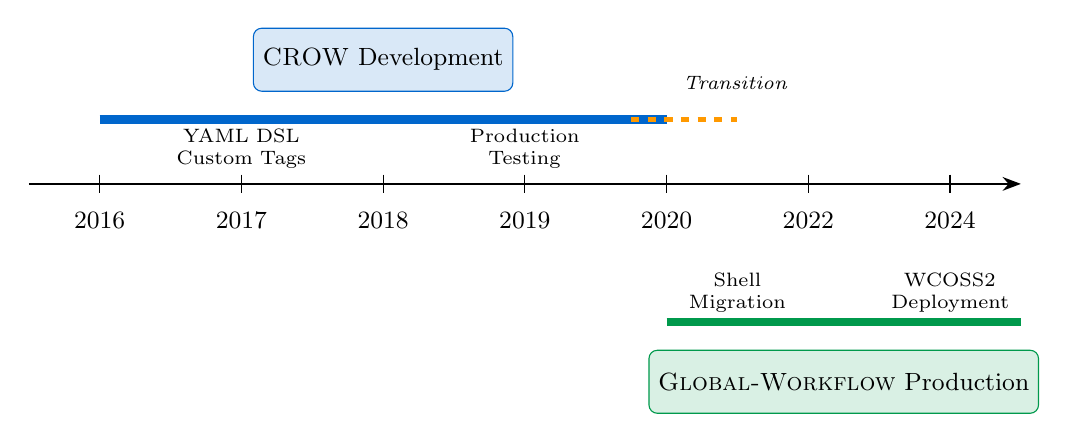
\begin{tikzpicture}[scale=0.9, yscale=1.3]
  % Timeline axis
  \draw[thick,-{Stealth}] (0,0) -- (14,0);
  
  % Year markers
  \foreach \x/\year in {1/2016, 3/2017, 5/2018, 7/2019, 9/2020, 11/2022, 13/2024} {
    \draw (\x,0.1) -- (\x,-0.1);
    \node[below] at (\x,-0.2) {\small \year};
  }
  
  % CROW era - above the timeline
  \draw[crowblue, line width=3pt] (1,0.7) -- (9,0.7);
  \node[crowbox, above] at (5,1.0) {\crow{} Development};
  \node[below, font=\scriptsize, text width=3cm, align=center] at (3,0.7) {YAML DSL\\Custom Tags};
  \node[below, font=\scriptsize, text width=3cm, align=center] at (7,0.7) {Production\\Testing};
  
  % Transition
  \draw[warnorange, line width=2pt, dashed] (8.5,0.7) -- (10,0.7);
  \node[right, font=\scriptsize\itshape] at (9.1,1.1) {Transition};
  
  % Global-Workflow era - well below the year markers
  \draw[gwgreen, line width=3pt] (9,-1.5) -- (14,-1.5);
  \node[gwbox, below] at (11.5,-1.8) {\gw{} Production};
  \node[above, font=\scriptsize, text width=2.5cm, align=center] at (10,-1.5) {Shell\\Migration};
  \node[above, font=\scriptsize, text width=2.5cm, align=center] at (13,-1.5) {WCOSS2\\Deployment};
  
\end{tikzpicture}
\caption{Timeline of resource configuration approaches at NOAA/EMC}
\label{fig:timeline}
\end{figure}

\subsection{Scope and Methodology}

This analysis draws from:
\begin{itemize}[leftmargin=2em]
    \item Primary source code from \texttt{NOAA-EMC/global-workflow} (current)
    \item Archived \crow{} codebase (\texttt{workflow/} directory, pre-2020)
    \item Platform configuration files for all production HPC systems
    \item Our companion \mpmd{} Runtime Infrastructure analysis (2025)
    \item Operational experience from forecast cycle deployments
\end{itemize}

We employ a structured comparison methodology, examining each system across four dimensions:
\begin{enumerate}
    \item \textbf{Specification}: How resources are defined
    \item \textbf{Validation}: How errors are detected
    \item \textbf{Execution}: How specifications become runtime behavior
    \item \textbf{Maintenance}: How changes propagate through the system
\end{enumerate}

\section{Resource Specification Paradigms}
\label{sec:paradigms}

\subsection{Architectural Overview}

Figure~\ref{fig:architecture} contrasts the data flow in both systems from resource definition to job submission.

\begin{figure}[H]
\centering
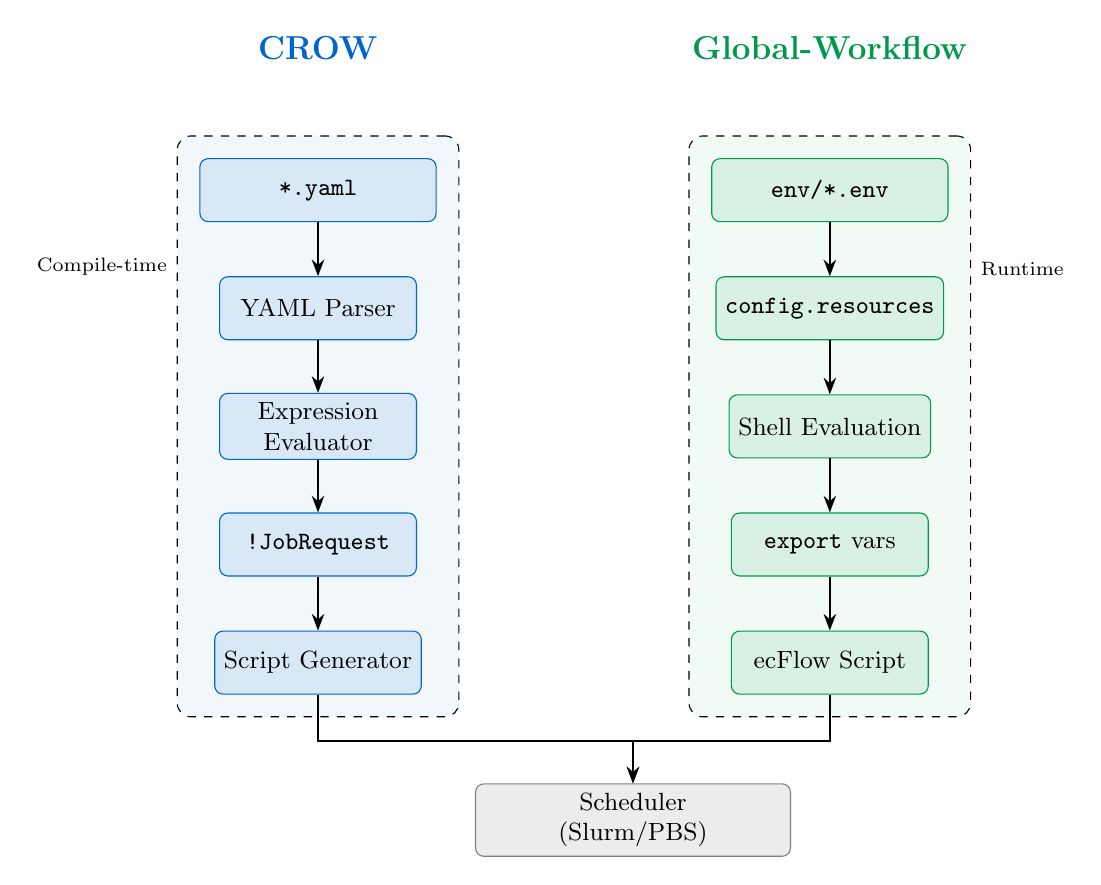
\begin{tikzpicture}[node distance=1.5cm]
  % CROW side
  \node[crowbox, minimum width=3cm] (yaml) {\texttt{*.yaml}};
  \node[crowbox, below of=yaml] (parser) {YAML Parser};
  \node[crowbox, below of=parser] (eval) {Expression\\Evaluator};
  \node[crowbox, below of=eval] (jobreq) {\texttt{!JobRequest}};
  \node[crowbox, below of=jobreq] (gen) {Script Generator};
  
  \draw[arrow] (yaml) -- (parser);
  \draw[arrow] (parser) -- (eval);
  \draw[arrow] (eval) -- (jobreq);
  \draw[arrow] (jobreq) -- (gen);
  
  % CROW label
  \node[above of=yaml, yshift=0.3cm, font=\bfseries\large, text=crowblue] {\crow{}};
  
  % GW side
  \node[gwbox, minimum width=3cm, right of=yaml, xshift=5cm] (env) {\texttt{env/*.env}};
  \node[gwbox, below of=env] (config) {\texttt{config.resources}};
  \node[gwbox, below of=config] (shell) {Shell Evaluation};
  \node[gwbox, below of=shell] (export) {\texttt{export} vars};
  \node[gwbox, below of=export] (ecf) {ecFlow Script};
  
  \draw[arrow] (env) -- (config);
  \draw[arrow] (config) -- (shell);
  \draw[arrow] (shell) -- (export);
  \draw[arrow] (export) -- (ecf);
  
  % GW label
  \node[above of=env, yshift=0.3cm, font=\bfseries\large, text=gwgreen] {\gw{}};
  
  % Shared output
  \node[sharedbox, below of=gen, xshift=4cm, yshift=-0.5cm, minimum width=4cm] (submit) {Scheduler\\(Slurm/PBS)};
  
  \draw[arrow] (gen) -- ++(0,-1) -| (submit);
  \draw[arrow] (ecf) -- ++(0,-1) -| (submit);
  
  % Background layer
  \begin{scope}[on background layer]
    \node[layer, fill=crowblue!5, fit=(yaml)(gen), label=above left:{\scriptsize Compile-time}] {};
    \node[layer, fill=gwgreen!5, fit=(env)(ecf), label=above right:{\scriptsize Runtime}] {};
  \end{scope}
  
\end{tikzpicture}
\caption{Architectural comparison: \crow{} (left) performs resolution at YAML parse time; \gw{} (right) resolves at shell evaluation time}
\label{fig:architecture}
\end{figure}

\subsection{CROW: Declarative Resource Tables}
\label{sec:crow-tables}

\crow{} centralized all resource definitions in \texttt{workflow/defaults/default\_resources.yaml} using resolution-indexed lookup tables with custom YAML type extensions.

\subsubsection{The Type System}

\crow{} extended standard YAML with custom tags forming a Domain-Specific Language (DSL):

\begin{table}[H]
\centering
\caption{\crow{} Custom YAML Tags}
\label{tab:crow-tags}
\begin{tabular}{@{}llp{7cm}@{}}
\toprule
\textbf{Tag} & \textbf{Type} & \textbf{Purpose} \\
\midrule
\texttt{!Select} & Pattern Match & Conditional selection based on configuration value \\
\texttt{!calc} & Expression & Deferred Python expression evaluation \\
\texttt{!icalc} & Immediate Calc & Immediate expression evaluation during parse \\
\texttt{!JobRequest} & Resource Spec & Structured job resource specification \\
\texttt{!timedelta} & Duration & Time duration with HH:MM:SS parsing \\
\texttt{!error} & Exception & Explicit failure for undefined cases \\
\texttt{!Platform} & Platform Def & HPC platform configuration container \\
\texttt{!FirstTrue} & Conditional & First matching condition selection \\
\bottomrule
\end{tabular}
\end{table}

\subsubsection{Resource Table Structure}

The core GFS resource table demonstrates \crow{}'s resolution-indexed approach:

\begin{lstlisting}[language=YAML, caption={\crow{} GFS Resource Table (from \texttt{default\_resources.yaml})}]
gfs_resource_table: !Select
  select: !icalc doc.fv3_gfs_settings.CASE
  otherwise: !error Unknown GFS case 
  cases:
    C96:  &gfs_resource_C96
      prep:     [  12,   12, !timedelta "00:15:00", null, null ]
      anal:     [ 144,    6, !timedelta "01:30:00", max, null  ]
      fcst:     [ 168,   12, !timedelta "00:30:00", 2, null    ]
      post:     [  84,   12, !timedelta "02:00:00", 1, null    ]
      vrfy:     [   1,    1, !timedelta "03:00:00", null, null ]
    C384: &gfs_resource_C384
      prep:     [   4,    4, !timedelta "00:15:00", max, null  ]
      anal:     [ 360,    6, !timedelta "01:30:00", max, null  ]
      fcst:     [ 384,    6, !timedelta "02:30:00", 4, null    ]
      post:     [ 240,    8, !timedelta "06:00:00", 1, null    ]
      vrfy:     [   3,    1, !timedelta "05:00:00", null, null ]
    C768: &gfs_resource_C768
      prep:     [   4,    4, !timedelta "00:15:00", max, null  ]
      anal:     [ 480,    6, !timedelta "02:30:00", max, null  ]
      fcst:     [ 768,    6, !timedelta "05:00:00", 4, null    ]
      post:     [ 480,    8, !timedelta "08:00:00", 1, null    ]
      vrfy:     [   5,    1, !timedelta "06:00:00", null, null ]
\end{lstlisting}

The tuple format follows a consistent schema:
\begin{equation}
\text{tuple} = [\text{ranks}, \text{ppn}, \text{walltime}, \text{threads}, \text{memory}]
\end{equation}

Where:
\begin{itemize}[leftmargin=2em]
    \item \textbf{ranks}: Total MPI processes
    \item \textbf{ppn}: Processes per node (determines node count: $\lceil \text{ranks}/\text{ppn} \rceil$)
    \item \textbf{walltime}: Maximum job duration (\texttt{!timedelta} parsed)
    \item \textbf{threads}: OpenMP threads per rank (\texttt{max} = all available, \texttt{null} = platform default)
    \item \textbf{memory}: Per-node memory limit (\texttt{null} = platform default)
\end{itemize}

\subsubsection{EnKF Resource Tables}

The ensemble Kalman filter required separate resource tables due to its different scaling characteristics:

\begin{lstlisting}[language=YAML, caption={\crow{} EnKF Resource Table}]
enkf_resource_table: !Select
  select: !icalc doc.fv3_gfs_settings.CASE
  otherwise: !error Unknown EnKF case
  cases:
    C384: &enkf_C384
      eobs:   [ 360, 6, !timedelta "00:30:00", null, null ]
      eomg:   [ 360, 6, !timedelta "01:00:00", null, null ]
      eupd:   [ 960, 6, !timedelta "00:35:00", 4, null    ]
      ecen:   [  80, 8, !timedelta "00:30:00", 2, null    ]
      esfc:   [  78, 6, !timedelta "00:10:00", null, null ]
      efcs:   [ 240, 6, !timedelta "02:30:00", 2, null    ]
    C768: &enkf_C768
      eobs:   [ 480, 6, !timedelta "00:45:00", null, null ]
      eomg:   [ 480, 6, !timedelta "01:30:00", null, null ]
      eupd:   [1200, 6, !timedelta "01:00:00", 4, null    ]
      ecen:   [ 120, 8, !timedelta "00:45:00", 2, null    ]
      esfc:   [ 156, 6, !timedelta "00:15:00", null, null ]
      efcs:   [ 384, 6, !timedelta "04:00:00", 2, null    ]
\end{lstlisting}

\subsubsection{JobRequest Construction}

Resources were consumed through \texttt{!JobRequest} objects that referenced the lookup tables:

\begin{lstlisting}[language=YAML, caption={\crow{} JobRequest Pattern}]
# Default JobRequest consuming gfs_resource_table
run_gdasfcst: !JobRequest
  - batch_memory: !icalc >-
      doc.gfs_resource_table.fcst[4]
  - mpi_ranks: !icalc >-
      doc.gfs_resource_table.fcst[0]
  - OMP_NUM_THREADS: !icalc >-
      doc.gfs_resource_table.fcst[3]
  - walltime: !icalc >-
      tools.to_timedelta(doc.gfs_resource_table.fcst[2])
  - OMP_STACKSIZE: !calc tools.OMP_STACKSIZE_default
  - max_ppn: !icalc >-
      doc.gfs_resource_table.fcst[1]

# Coupled model with different resources
run_coupled_fcst: !JobRequest
  - batch_memory: !icalc >-
      doc.coupled_resource_table.fcst[4]
  - mpi_ranks: !icalc >-
      doc.coupled_resource_table.fcst[0]
  - walltime: !icalc >-
      tools.to_timedelta(doc.coupled_resource_table.fcst[2])
  - OMP_NUM_THREADS: !icalc >-
      doc.coupled_resource_table.fcst[3] or 1
  - max_ppn: !icalc >-
      doc.coupled_resource_table.fcst[1]
\end{lstlisting}

\subsubsection{Downstream Resource Tables}

Post-processing and product generation jobs had different resource profiles:

\begin{minipage}{\linewidth}
\begin{lstlisting}[language=YAML, caption={\crow{} Downstream Resources}]
downstream_resource_table: !Select
  select: !icalc doc.fv3_gfs_settings.CASE
  otherwise: !error Unknown downstream case
  cases:
    C96:
      awips_g1:   [ 24, 24, !timedelta "00:05:00", 1, !calc memory.per_node ]
      awips_g2:   [ 24, 24, !timedelta "00:05:00", 1, !calc memory.per_node ]
      gempak:     [ 24, 24, !timedelta "00:05:00", 1, !calc memory.per_node ]
      bufrsnd:    [ 80,  8, !timedelta "00:20:00", 1, !calc memory.per_node ]
      postsnd:    [ 12, 12, !timedelta "00:30:00", 1, !calc memory.per_node ]
    C768:
      awips_g1:   [ 24, 24, !timedelta "00:10:00", 1, !calc memory.per_node ]
      awips_g2:   [ 24, 24, !timedelta "00:10:00", 1, !calc memory.per_node ]
      gempak:     [ 24, 24, !timedelta "00:10:00", 1, !calc memory.per_node ]
      bufrsnd:    [ 80,  8, !timedelta "00:45:00", 1, !calc memory.per_node ]
      postsnd:    [ 24, 12, !timedelta "01:00:00", 1, !calc memory.per_node ]
\end{lstlisting}
\end{minipage}

\subsection{Global-Workflow: Imperative Configuration}
\label{sec:gw-config}

The current \gw{} system employs a three-level configuration hierarchy using shell scripts with conditional logic.

\subsubsection{Configuration Hierarchy}

\begin{figure}[H]
\centering
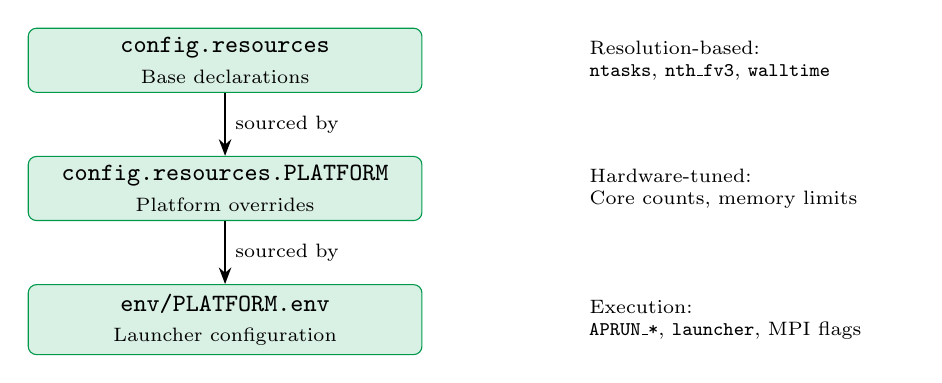
\begin{tikzpicture}[node distance=0.8cm]
  % Level 1
  \node[gwbox, minimum width=5cm] (base) {
    \texttt{config.resources}\\
    \scriptsize Base declarations
  };
  
  % Level 2
  \node[gwbox, minimum width=5cm, below=of base] (specific) {
    \texttt{config.resources.PLATFORM}\\
    \scriptsize Platform overrides
  };
  
  % Level 3
  \node[gwbox, minimum width=5cm, below=of specific] (env) {
    \texttt{env/PLATFORM.env}\\
    \scriptsize Launcher configuration
  };
  
  % Arrows with labels
  \draw[arrow] (base) -- node[right, font=\scriptsize] {sourced by} (specific);
  \draw[arrow] (specific) -- node[right, font=\scriptsize] {sourced by} (env);
  
  % Side annotations
  \node[right=2cm of base, font=\scriptsize, text width=4cm] {
    Resolution-based: \\
    \texttt{ntasks}, \texttt{nth\_fv3}, \texttt{walltime}
  };
  
  \node[right=2cm of specific, font=\scriptsize, text width=4cm] {
    Hardware-tuned: \\
    Core counts, memory limits
  };
  
  \node[right=2cm of env, font=\scriptsize, text width=4cm] {
    Execution: \\
    \texttt{APRUN\_*}, \texttt{launcher}, MPI flags
  };
  
\end{tikzpicture}
\caption{Three-level \gw{} configuration hierarchy}
\label{fig:gw-hierarchy}
\end{figure}

\subsubsection{Base Resource Configuration}

The primary resource file uses nested case statements for resolution and step:

\begin{lstlisting}[language=Bash, caption={\gw{} Base Resource Configuration (\texttt{config.resources})}]
#!/bin/bash

# Forecast resources by resolution
case "${step}" in
  "fcst"|"efcs")
    export layout_x="--layout_x"
    export layout_y="--layout_y"
    
    case "${CASE}" in
      "C48")
        export layout_x=1
        export layout_y=1
        export ntasks_fv3=6
        export ntasks_quilt=6
        export nth_fv3=2
        export nth_quilt=1
        export walltime="00:30:00"
        ;;
      "C96")
        export layout_x=4
        export layout_y=4
        export ntasks_fv3=96
        export ntasks_quilt=24
        export nth_fv3=2
        export nth_quilt=1
        export walltime="01:00:00"
        ;;
      "C384")
        export layout_x=8
        export layout_y=8
        export ntasks_fv3=384
        export ntasks_quilt=72
        export nth_fv3=4
        export nth_quilt=1
        export walltime="02:30:00"
        ;;
      "C768")
        export layout_x=12
        export layout_y=12
        export ntasks_fv3=864
        export ntasks_quilt=144
        export nth_fv3=4
        export nth_quilt=1
        export walltime="05:00:00"
        ;;
      "C1152")
        export layout_x=16
        export layout_y=16
        export ntasks_fv3=1536
        export ntasks_quilt=192
        export nth_fv3=4
        export nth_quilt=1
        export walltime="08:00:00"
        ;;
    esac
    
    # Total tasks = FV3 + Quilt
    export ntasks=$((ntasks_fv3 + ntasks_quilt))
    ;;
    
  "anal"|"analcalc"|"analdiag")
    case "${CASE}" in
      "C48")  export ntasks=60  ; export nth=4  ;;
      "C96")  export ntasks=120 ; export nth=8  ;;
      "C384") export ntasks=480 ; export nth=8  ;;
      "C768") export ntasks=960 ; export nth=8  ;;
    esac
    export walltime="${walltime_anal:-02:00:00}"
    ;;
    
  "post"|"postanl")
    case "${CASE}" in
      "C48")  export ntasks=24  ; export nth=1 ;;
      "C96")  export ntasks=84  ; export nth=1 ;;
      "C384") export ntasks=240 ; export nth=1 ;;
      "C768") export ntasks=480 ; export nth=1 ;;
    esac
    ;;
esac

# Memory calculation
export memory="${memory:-$((ntasks * 4))}GB"
\end{lstlisting}

\subsubsection{Platform-Specific Overrides}

Each platform can override base resources for hardware optimization:

\begin{lstlisting}[language=Bash, caption={Platform Override (\texttt{config.resources.HERA})}]
#!/bin/bash
# HERA-specific resource overrides

source "${HOMEgfs}/parm/config/config.resources"

# Hera has 40 cores/node - adjust ppn
case "${step}" in
  "fcst")
    export ppn=20  # Leave room for I/O
    export NTHREADS_FV3=${nth_fv3:-4}
    ;;
  "anal")
    export ppn=10  # Heavy memory per rank
    ;;
esac

# Memory constraints (Hera has 384GB/node)
export memory="180GB"
\end{lstlisting}

\subsubsection{Platform Environment Files}

The final layer configures MPI launchers and execution parameters:

\begin{lstlisting}[language=Bash, caption={HERA Platform Environment (\texttt{env/HERA.env})}]
#!/bin/bash
# HERA - Slurm/Intel MPI Configuration

# System limits
ulimit -s unlimited
ulimit -a

# Launcher configuration
launcher="srun -l --export=ALL"
mpmd_opt="--multi-prog"

# MPI tuning for Intel MPI
export I_MPI_EXTRA_FILESYSTEM=on
export I_MPI_EXTRA_FILESYSTEM_FORCE=gpfs
export I_MPI_ADJUST_ALLREDUCE=5

# Construct APRUN commands per component
case "${step}" in
  "fcst"|"efcs")
    export APRUN_UFS="${launcher} -n ${ntasks}"
    export APRUN_FV3="${launcher} -n ${ntasks_fv3} --cpus-per-task=${nth_fv3}"
    ;;
  "anal"|"analcalc")
    export APRUN_GSI="${launcher} -n ${ntasks} --cpus-per-task=${nth}"
    ;;
  "post"|"postanl")
    export APRUN_UPP="${launcher} -n ${ntasks}"
    ;;
  "prep"|"prepbufr")
    export APRUN_PREP="${launcher} -n 4"
    ;;
esac

# Generic commands
export APRUN_GAUSSIAN="${launcher} -n ${ntasks} --cpus-per-task=${nth:-1}"
export APRUN_CHGRES="${launcher} -n 6"
export APRUN_REGRID="${launcher} -n ${ntasks}"
\end{lstlisting}

\begin{lstlisting}[language=Bash, caption={WCOSS2 Platform Environment (\texttt{env/WCOSS2.env})}]
#!/bin/bash
# WCOSS2 - PBS Pro/Cray MPICH Configuration

# System limits
ulimit -s unlimited
ulimit -a

# Cray-specific settings
export MPICH_MPIIO_HINTS_DISPLAY=1
export MALLOC_MMAP_MAX_=0
export MALLOC_TRIM_THRESHOLD_=134217728

# PBS Pro launcher
launcher="mpiexec -l"
launcher_CFP="mpiexec -np \${nprocs} --cpu-bind verbose,core cfp"
mpmd_opt="--cpu-bind verbose,core cfp"

# Module loading for CFP
module load cfp/2.0.4 || true

# APRUN construction 
case "${step}" in
  "fcst"|"efcs")
    export APRUN_UFS="${launcher} -np ${ntasks} --cpu-bind core"
    export APRUN_FV3="${launcher} -np ${ntasks_fv3} --depth ${nth_fv3}"
    ;;
  "anal"|"analcalc")
    export APRUN_GSI="${launcher} -np ${ntasks} --depth ${nth}"
    ;;
  "post"|"postanl")
    export APRUN_UPP="${launcher} -np ${ntasks}"
    ;;
esac
\end{lstlisting}

\subsubsection{ecFlow Job Script Integration}

Resources flow into ecFlow job scripts through variable substitution:

\begin{lstlisting}[language=Bash, caption={ecFlow Job Script Header}]
#!/bin/bash
#PBS -N %JOBNAME%
#PBS -A %ACCOUNT%
#PBS -q %QUEUE%
#PBS -l walltime=%WALLTIME%
#PBS -l select=%NODES%:ncpus=%NCPUS%:mem=%MEMORY%
#PBS -l place=scatter
#PBS -j oe
#PBS -o %COM%/logs/%PDY%/%CYCINC%/%JOBNAME%.log

# Or for Slurm:
#SBATCH --job-name=%JOBNAME%
#SBATCH --account=%ACCOUNT%
#SBATCH --partition=%QUEUE%
#SBATCH --time=%WALLTIME%
#SBATCH --nodes=%NODES%
#SBATCH --ntasks=%NTASKS%
#SBATCH --cpus-per-task=%NCPUS%
#SBATCH --mem=%MEMORY%
#SBATCH --output=%COM%/logs/%PDY%/%CYCINC%/%JOBNAME%.log

# Source configuration hierarchy
source "${HOMEgfs}/parm/config/config.base"
source "${HOMEgfs}/parm/config/config.resources"
source "${HOMEgfs}/env/${machine}.env"
\end{lstlisting}

\section{MPI Execution Patterns}
\label{sec:mpi}

This section integrates findings from our companion \mpmd{} Runtime Infrastructure analysis, examining how both systems translate resource specifications into actual MPI execution.

\subsection{The SPMD/MPMD Dichotomy}

\begin{figure}[H]
\centering
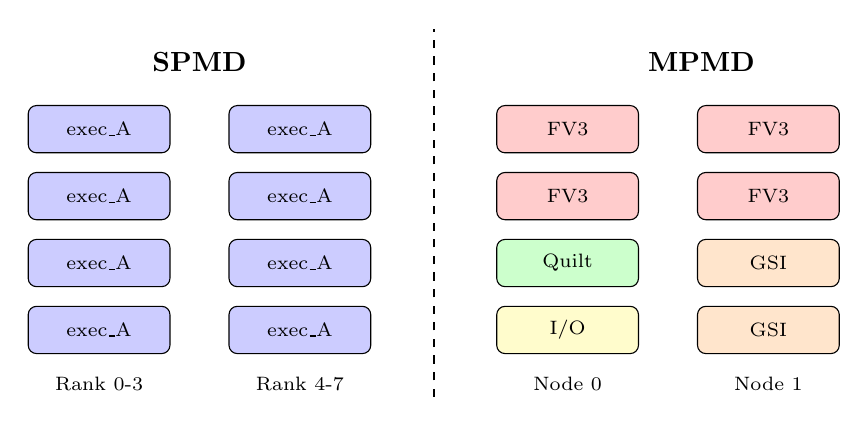
\begin{tikzpicture}[scale=0.85]
  % SPMD side
  \node[font=\bfseries] at (2.5,4) {SPMD};
  
  \foreach \y in {0,1,2,3} {
    \node[box, fill=blue!20, minimum width=1.8cm, minimum height=0.6cm] at (1,\y) {\scriptsize exec\_A};
    \node[box, fill=blue!20, minimum width=1.8cm, minimum height=0.6cm] at (4,\y) {\scriptsize exec\_A};
  }
  
  \node[font=\scriptsize] at (1,-0.8) {Rank 0-3};
  \node[font=\scriptsize] at (4,-0.8) {Rank 4-7};
  
  % MPMD side  
  \node[font=\bfseries] at (10,4) {MPMD};
  
  \node[box, fill=red!20, minimum width=1.8cm, minimum height=0.6cm] at (8,3) {\scriptsize FV3};
  \node[box, fill=red!20, minimum width=1.8cm, minimum height=0.6cm] at (8,2) {\scriptsize FV3};
  \node[box, fill=green!20, minimum width=1.8cm, minimum height=0.6cm] at (8,1) {\scriptsize Quilt};
  \node[box, fill=yellow!20, minimum width=1.8cm, minimum height=0.6cm] at (8,0) {\scriptsize I/O};
  
  \node[box, fill=red!20, minimum width=1.8cm, minimum height=0.6cm] at (11,3) {\scriptsize FV3};
  \node[box, fill=red!20, minimum width=1.8cm, minimum height=0.6cm] at (11,2) {\scriptsize FV3};
  \node[box, fill=orange!20, minimum width=1.8cm, minimum height=0.6cm] at (11,1) {\scriptsize GSI};
  \node[box, fill=orange!20, minimum width=1.8cm, minimum height=0.6cm] at (11,0) {\scriptsize GSI};
  
  \node[font=\scriptsize] at (8,-0.8) {Node 0};
  \node[font=\scriptsize] at (11,-0.8) {Node 1};
  
  % Separator
  \draw[thick, dashed] (6,-1) -- (6,4.5);
  
\end{tikzpicture}
\caption{SPMD (single program) vs MPMD (multiple programs) execution models}
\label{fig:spmd-mpmd}
\end{figure}

\subsection{CROW: Abstract Parallelism Layer}
\label{sec:crow-parallel}

\crow{} generated scheduler-agnostic job specifications through platform configuration files that abstracted the execution model.

\subsubsection{Platform Definition}

\begin{lstlisting}[language=YAML, caption={\crow{} Hera Platform Configuration}]
hera: !Platform
  name: hera
  physical_cores_per_node: 40
  hyperthreading_allowed: true
  logical_cores_per_node: 80
  
  scheduler_settings: !icalc |
    tools.get_scheduler(
      sched='Slurm',
      machine='hera',
      partition='hera')
  
  partitions:
    default: &default_partition
      specification: !icalc |
        tools.get_parallelism('HydraIMPI')
      scheduler_settings:
        partition: hera
        qos: batch
        account: !calc doc.platform.accounting.account
        
    bigmem:
      specification: !icalc |
        tools.get_parallelism('HydraIMPI')  
      scheduler_settings:
        partition: bigmem
        qos: batch
        
    service:
      specification: !icalc |
        tools.get_parallelism('LocalSerial')
      scheduler_settings:
        partition: service
        qos: batch
  
  parallelism: !calc |
    tools.get_parallelism('HydraIMPI')
    
  scheduler: !calc |
    tools.get_scheduler('Slurm')
    
  nodes: !calc |
    tools.get_node_count(
      doc.platform.physical_cores_per_node,
      hyperthreading=True)
\end{lstlisting}

\subsubsection{WCOSS Configuration (Historical)}

\begin{lstlisting}[language=YAML, caption={\crow{} WCOSS Dell P3 Configuration}]
wcoss_dell_p3: !Platform
  name: wcoss_dell_p3
  physical_cores_per_node: 28
  hyperthreading_allowed: false
  
  scheduler_settings: !icalc |
    tools.get_scheduler(
      sched='LSF',
      machine='dell_p3')
  
  use_task_geometry: false  # CFP mode
  
  partitions:
    default:
      specification: !icalc |
        tools.get_parallelism('LSFpoe')
      scheduler_settings:
        partition: !FirstTrue
          - when: !calc tools.can_write('/gpfs/hps2/ptmp/')
            do: dev
          - otherwise: devmax
        account: !calc doc.platform.accounting.account
        
    transfer:
      specification: !icalc |
        tools.get_parallelism('LocalSerial')
      scheduler_settings:
        partition: transfer
        
  # CFP module for MPMD
  rocoto_load_modules: |
    module load cfp
    module load ics
\end{lstlisting}

Algorithm~\ref{alg:crow-resolution} describes how \crow{} resolved resource specifications:

\begin{algorithm}[H]
\caption{\crow{} Resource Resolution}
\label{alg:crow-resolution}
\begin{algorithmic}[1]
\REQUIRE YAML configuration tree $D$, platform $P$, job $J$
\ENSURE Scheduler-specific job script
\STATE $\text{CASE} \gets D.\text{fv3\_gfs\_settings.CASE}$ \COMMENT{Get resolution}
\STATE $\text{table} \gets$ SELECT($D.\text{gfs\_resource\_table}, \text{CASE}$)
\IF{table = \texttt{!error}}
    \STATE \textbf{raise} ConfigurationError
\ENDIF
\STATE $\text{tuple} \gets \text{table}[J.\text{step}]$ \COMMENT{[ranks, ppn, wall, threads, mem]}
\STATE $\text{req} \gets$ BuildJobRequest(tuple)
\STATE $\text{sched} \gets P.\text{scheduler\_settings.scheduler\_name}$
\STATE $\text{script} \gets$ GenerateScript(req, sched, $P$)
\RETURN script
\end{algorithmic}
\end{algorithm}

\subsection{Global-Workflow: MPMD Wrapper System}
\label{sec:gw-mpmd}

The current \gw{} system uses \texttt{ush/run\_mpmd.sh} as a unified interface for \mpmd{} execution across schedulers.

\subsubsection{MPMD Execution Architecture}

\begin{figure}[H]
\centering
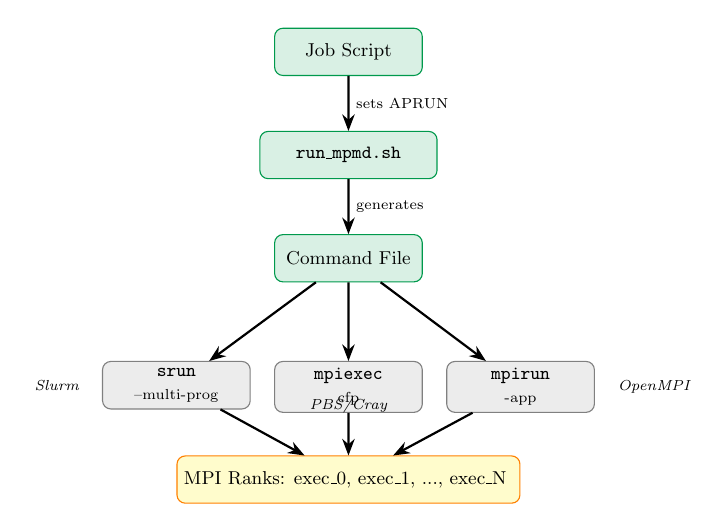
\begin{tikzpicture}[node distance=0.7cm, scale=0.75, every node/.style={scale=0.75}]
  % Script layer
  \node[gwbox] (script) {Job Script};
  
  % run_mpmd.sh
  \node[gwbox, below=of script, minimum width=3cm] (mpmd) {\texttt{run\_mpmd.sh}};
  
  % Command file
  \node[gwbox, below=of mpmd] (cmdfile) {Command File};
  
  % Platform detection
  \node[sharedbox, below left=1cm and 0.3cm of cmdfile] (srun) {
    \texttt{srun}\\
    \scriptsize --multi-prog
  };
  \node[sharedbox, below=1cm of cmdfile] (mpiexec) {
    \texttt{mpiexec}\\
    \scriptsize cfp
  };
  \node[sharedbox, below right=1cm and 0.3cm of cmdfile] (orte) {
    \texttt{mpirun}\\
    \scriptsize -app
  };
  
  % MPI execution
  \node[dbbox, below=2.2cm of cmdfile, minimum width=5cm] (ranks) {
    MPI Ranks: exec\_0, exec\_1, ..., exec\_N
  };
  
  % Connections
  \draw[arrow] (script) -- node[right, font=\scriptsize] {sets APRUN} (mpmd);
  \draw[arrow] (mpmd) -- node[right, font=\scriptsize] {generates} (cmdfile);
  \draw[arrow] (cmdfile) -- (srun);
  \draw[arrow] (cmdfile) -- (mpiexec);
  \draw[arrow] (cmdfile) -- (orte);
  \draw[arrow] (srun) -- (ranks);
  \draw[arrow] (mpiexec) -- (ranks);
  \draw[arrow] (orte) -- (ranks);
  
  % Platform labels
  \node[left=0.2cm of srun, font=\scriptsize\itshape] {Slurm};
  \node[below=0.1cm of mpiexec, font=\scriptsize\itshape, yshift=0.5cm] {PBS/Cray};
  \node[right=0.2cm of orte, font=\scriptsize\itshape] {OpenMPI};
  
\end{tikzpicture}
\caption{\gw{} \mpmd{} execution flow through \texttt{run\_mpmd.sh}}
\label{fig:mpmd-flow}
\end{figure}

\subsubsection{Command File Generation}

\begin{lstlisting}[language=Bash, caption={\texttt{run\_mpmd.sh} Core Functions}]
#!/bin/bash
# run_mpmd.sh - Unified MPMD execution wrapper

# Generate MPMD command file
# Arguments: pairs of (nprocs, command)
# Output: cmdfile with one line per MPI rank
create_mpmd_cmdfile() {
    local cmdfile=$1
    shift
    
    > "${cmdfile}"  # Truncate
    local rank=0
    
    while (( $# >= 2 )); do
        local nprocs=$1
        local cmd=$2
        shift 2
        
        for (( i=0; i<nprocs; i++ )); do
            if [[ "${SCHEDULER}" == "slurm" ]]; then
                # Slurm multi-prog format: rank command
                echo "${rank} ${cmd}" >> "${cmdfile}"
            else
                # PBS/cfp format: command only
                echo "${cmd}" >> "${cmdfile}"
            fi
            ((rank++))
        done
    done
    
    echo "Generated ${rank} rank entries in ${cmdfile}" >&2
}

# Execute MPMD job
run_mpmd() {
    local cmdfile=$1
    local total_ranks=$2
    
    case "${launcher_type:-srun}" in
        "srun")
            # Slurm: srun with --multi-prog
            ${APRUN_MPMD:-srun} \
                -n "${total_ranks}" \
                --multi-prog "${cmdfile}"
            ;;
        "mpiexec"|"mpiexec_mpt")
            # PBS/Cray: mpiexec with cfp
            module load cfp 2>/dev/null || true
            ${APRUN_MPMD:-mpiexec} \
                -np "${total_ranks}" \
                --cpu-bind verbose,core \
                cfp "${cmdfile}"
            ;;
        "mpirun")
            # OpenMPI: mpirun with -app
            ${APRUN_MPMD:-mpirun} \
                -np "${total_ranks}" \
                -app "${cmdfile}"
            ;;
        *)
            echo "ERROR: Unknown launcher_type: ${launcher_type}" >&2
            return 1
            ;;
    esac
}
\end{lstlisting}

\subsubsection{CFP (Coupled Framework Parallelism)}

The \cfp{} module enables \mpmd{} execution on \textsc{WCOSS2}:

\begin{lstlisting}[language=Bash, caption={CFP Command File Format}]
# cmdfile.mpmd - One command per MPI rank
# Ranks 0-95: FV3 atmospheric model
/path/to/ufs_weather_model
/path/to/ufs_weather_model
... (96 lines)
# Ranks 96-119: Quilt/Write component  
/path/to/ufs_weather_model --write
/path/to/ufs_weather_model --write
... (24 lines)
# Ranks 120-123: Post-processor
/path/to/ncep_post
/path/to/ncep_post
/path/to/ncep_post
/path/to/ncep_post
\end{lstlisting}

\subsection{Launcher Abstraction Comparison}

Both systems abstract the launcher, but at different levels:

\begin{table}[H]
\centering
\caption{Launcher Abstraction Comparison}
\label{tab:launcher-compare}
\begin{tabular}{@{}p{3.2cm}p{4.5cm}p{4.8cm}@{}}
\toprule
\textbf{Aspect} & \textbf{\crow{}} & \textbf{\gw{}} \\
\midrule
Abstraction level & YAML configuration & Shell variables \\
Resolution time & YAML parse & Runtime \\
Slurm command & Generated by \texttt{!Platform} & \texttt{\$\{launcher\} = "srun -l"} \\
PBS command & Generated by \texttt{!Platform} & \texttt{\$\{launcher\} = "mpiexec -l"} \\
MPMD syntax & Generated from \texttt{!JobRequest} & Manual cmdfile via \texttt{run\_mpmd.sh} \\
Thread binding & \texttt{tools.get\_parallelism()} & \texttt{--cpus-per-task}, \texttt{--depth} \\
\bottomrule
\end{tabular}
\end{table}

\section{Comparative Analysis}
\label{sec:comparison}

This section provides a structured comparison across the four dimensions identified in Section~\ref{sec:introduction}.

\subsection{Code Organization}

Table~\ref{tab:file_organization} compares where resource information resides in each system.

\begin{table}[H]
\centering
\caption{File Organization Comparison}
\label{tab:file_organization}
\begin{tabular}{@{}p{3.2cm}p{4.2cm}p{5.2cm}@{}}
\toprule
\textbf{Component} & \textbf{\crow{}} & \textbf{\gw{}} \\
\midrule
Resource definitions & \texttt{workflow/defaults/}\newline\texttt{default\_resources.yaml} & \texttt{parm/config/config.resources} \\
\addlinespace
Platform config & \texttt{workflow/platforms/}\newline\texttt{*.yaml} & \texttt{env/*.env} \\
\addlinespace
Platform overrides & Inherited via YAML & \texttt{parm/config/config.resources.*} \\
\addlinespace
Scheduler headers & Generated at parse time & \texttt{ecf/scripts/*.ecf} (embedded) \\
\addlinespace
MPMD handling & Via \texttt{!JobRequest} composition & \texttt{ush/run\_mpmd.sh} \\
\addlinespace
MPI tuning & In platform YAML & In \texttt{env/*.env} \\
\bottomrule
\end{tabular}
\end{table}

\subsection{Adding a New Resolution}

\subsubsection{CROW Approach}

Add one entry to each resource table:

\begin{lstlisting}[language=YAML, caption={Adding C1152 to \crow{}}]
gfs_resource_table: !Select
  select: !icalc doc.fv3_gfs_settings.CASE
  cases:
    # ... existing cases ...
    C1152: &gfs_resource_C1152
      prep:  [   6,    6, !timedelta "00:20:00", max, null ]
      anal:  [ 720,    6, !timedelta "03:30:00", max, null ]
      fcst:  [1536,    6, !timedelta "08:00:00", 4, null   ]
      post:  [ 720,    8, !timedelta "10:00:00", 1, null   ]
      vrfy:  [   8,    1, !timedelta "08:00:00", null, null]
\end{lstlisting}

\textbf{Propagation}: All jobs using \texttt{gfs\_resource\_table} automatically inherit the new resolution. The \texttt{!JobRequest} objects require no modification.

\textbf{Lines changed}: $\sim$6 (one table entry)

\subsubsection{Global-Workflow Approach}

Add case branches to each step in \texttt{config.resources}:

\begin{lstlisting}[language=Bash, caption={Adding C1152 to \gw{}}]
case "${step}" in
  "fcst"|"efcs")
    case "${CASE}" in
      # ... existing cases ...
      "C1152")
        export layout_x=16
        export layout_y=16
        export ntasks_fv3=1536
        export ntasks_quilt=192
        export nth_fv3=4
        export nth_quilt=1
        export walltime="08:00:00"
        ;;
    esac
    ;;
  "anal"|"analcalc"|"analdiag")
    case "${CASE}" in
      # ... existing cases ...
      "C1152")
        export ntasks=720
        export nth=8
        export walltime="03:30:00"
        ;;
    esac
    ;;
  "post"|"postanl")
    case "${CASE}" in
      # ... existing cases ...
      "C1152")
        export ntasks=720
        export nth=1
        ;;
    esac
    ;;
  # ... repeat for 15+ additional steps ...
esac
\end{lstlisting}

\textbf{Propagation}: Each step must be updated independently. Missing a step may cause runtime failures or incorrect resource allocation.

\textbf{Lines changed}: $\sim$50-100 (depending on step count)

\subsection{Adding a New HPC Platform}

\subsubsection{CROW Approach}

Create a new platform YAML file:

\begin{lstlisting}[language=YAML, caption={New Platform in \crow{}}]
# workflow/platforms/aws_pcluster.yaml
aws_pcluster: !Platform
  name: aws_pcluster
  physical_cores_per_node: 96  # c6i.24xlarge
  hyperthreading_allowed: true
  logical_cores_per_node: 192
  
  scheduler_settings: !icalc |
    tools.get_scheduler(
      sched='Slurm',
      machine='aws_pcluster')
  
  partitions:
    compute:
      specification: !icalc |
        tools.get_parallelism('PMI2')
      scheduler_settings:
        partition: compute
        account: !calc doc.platform.accounting.account
        
    spot:
      specification: !icalc |
        tools.get_parallelism('PMI2')
      scheduler_settings:
        partition: spot
        
  parallelism: !calc tools.get_parallelism('PMI2')
  scheduler: !calc tools.get_scheduler('Slurm')
\end{lstlisting}

\textbf{Files changed}: 1 new file

\subsubsection{Global-Workflow Approach}

Create multiple files:

\begin{lstlisting}[language=Bash, caption={New Platform Environment (\texttt{env/AWS.env})}]
#!/bin/bash
# AWS ParallelCluster - Slurm/PMI2 Configuration

ulimit -s unlimited

# PMI2 settings for AWS
export I_MPI_PMI_LIBRARY=/opt/slurm/lib/libpmi2.so
export I_MPI_FABRICS=shm:ofi
export FI_PROVIDER=efa

launcher="srun -l --export=ALL --mpi=pmi2"
mpmd_opt="--multi-prog"

# APRUN for each step (15+ definitions)
case "${step}" in
  "fcst"|"efcs")
    export APRUN_UFS="${launcher} -n ${ntasks}"
    export APRUN_FV3="${launcher} -n ${ntasks_fv3}"
    ;;
  "anal"|"analcalc")
    export APRUN_GSI="${launcher} -n ${ntasks}"
    ;;
  # ... 10+ more cases ...
esac
\end{lstlisting}

\begin{lstlisting}[language=Bash, caption={Platform Resource Overrides (\texttt{config.resources.AWS})}]
#!/bin/bash
# AWS-specific resource tuning

source "${HOMEgfs}/parm/config/config.resources"

# AWS c6i.24xlarge: 96 cores, 192GB
case "${step}" in
  "fcst")
    export ppn=24  # 4 ranks * 4 threads = 96 
    ;;
  "anal")
    export ppn=12  # Heavy memory per rank
    ;;
esac

export memory="180GB"
\end{lstlisting}

Additionally, update ecFlow templates with AWS-specific headers.

\textbf{Files changed}: 2-3 new files + template modifications

\subsection{Validation Capabilities}

\begin{table}[H]
\centering
\caption{Validation Feature Comparison}
\label{tab:validation}
\begin{tabular}{@{}lcc@{}}
\toprule
\textbf{Feature} & \textbf{\crow{}} & \textbf{\gw{}} \\
\midrule
Schema validation & Yes (YAML) & No \\
Type checking & Yes (custom tags) & No \\
Undefined case detection & \texttt{!error} at parse & Runtime default \\
Expression syntax errors & Parse-time & Runtime \\
Missing variable detection & Parse-time & Runtime (or silent) \\
Cross-reference validation & Yes (doc refs) & No \\
Static analysis possible & Yes & Limited \\
IDE syntax support & Limited & Excellent \\
Syntax highlighting & YAML-based & Full Bash \\
Linting tools & Custom & ShellCheck \\
\bottomrule
\end{tabular}
\end{table}

\subsection{Error Handling Patterns}

\subsubsection{CROW: Fail-Fast}

\begin{lstlisting}[language=YAML, caption={\crow{} Error Handling}]
gfs_resource_table: !Select
  select: !icalc doc.settings.CASE
  otherwise: !error |
    Unknown resolution '{{doc.settings.CASE}}'.
    Supported: C96, C192, C384, C768
  cases:
    C96: [...]
    C384: [...]
    C768: [...]
\end{lstlisting}

\textbf{Behavior}: Invalid configurations fail at YAML parse time, before job submission. Error messages include context.

\subsubsection{Global-Workflow: Defensive Defaults}

\begin{lstlisting}[language=Bash, caption={\gw{} Default Handling}]
case "${CASE}" in
  "C96")  export ntasks=48  ;;
  "C384") export ntasks=150 ;;
  "C768") export ntasks=360 ;;
  *)
    echo "WARNING: Unknown CASE '${CASE}', using default" >&2
    export ntasks=${ntasks:-24}  # Fallback
    ;;
esac
\end{lstlisting}

\textbf{Behavior}: Unknown configurations proceed with potentially incorrect defaults. May cause job failures or resource waste.

\subsection{Maintenance Metrics}

\begin{table}[H]
\centering
\caption{Lines of Code for Resource Configuration}
\label{tab:loc}
\begin{tabular}{@{}lrrl@{}}
\toprule
\textbf{Component} & \textbf{\crow{}} & \textbf{\gw{}} & \textbf{Notes} \\
\midrule
Core resource definitions & $\sim$350 & $\sim$1,200 & Resolution tables vs case statements \\
Platform config (per platform) & $\sim$60 & $\sim$150 & YAML vs shell + headers \\
JobRequest constructors & $\sim$200 & N/A & Reusable patterns \\
MPMD wrapper & N/A & $\sim$150 & \texttt{run\_mpmd.sh} \\
\midrule
\textbf{Total (6 platforms)} & $\sim$910 & $\sim$2,250 & \\
\bottomrule
\end{tabular}
\end{table}

\begin{table}[H]
\centering
\caption{Change Propagation Analysis}
\label{tab:propagation}
\begin{tabular}{@{}p{4cm}cc@{}}
\toprule
\textbf{Change Type} & \textbf{\crow{} Files} & \textbf{\gw{} Files} \\
\midrule
New resolution (C1152) & 1 & 1-2 \\
New platform & 1 & 2-3 \\
New step type & 1-2 & 3-5 \\
Walltime adjustment (global) & 1 & 15+ \\
Memory limit change & 1 & 6+ \\
Thread count change & 1 & 15+ \\
\bottomrule
\end{tabular}
\end{table}

\section{Resource Tuple Semantics}
\label{sec:semantics}

Both systems encode the same fundamental resource parameters, but with different representations and semantics.

\subsection{CROW Tuple Format}

\crow{}'s fixed-position tuples provide a compact, position-dependent encoding:

\begin{equation}
\text{tuple} = [\text{ranks}, \text{ppn}, \text{walltime}, \text{threads}, \text{memory}]
\end{equation}

\begin{table}[H]
\centering
\caption{\crow{} Tuple Field Semantics}
\label{tab:crow-tuple}
\begin{tabular}{@{}clp{6cm}l@{}}
\toprule
\textbf{Index} & \textbf{Field} & \textbf{Meaning} & \textbf{Special Values} \\
\midrule
0 & ranks & Total MPI processes & Integer \\
1 & ppn & Processes per node & Integer \\
2 & walltime & HH:MM:SS duration & \texttt{!timedelta} object \\
3 & threads & OpenMP threads/rank & \texttt{max}, \texttt{null}, Integer \\
4 & memory & Per-node memory & \texttt{null}, String (e.g., \texttt{"4G"}) \\
\bottomrule
\end{tabular}
\end{table}

\textbf{Node calculation}:
\begin{equation}
\text{nodes} = \left\lceil \frac{\text{ranks}}{\text{ppn}} \right\rceil
\end{equation}

\textbf{Example}: \texttt{[240, 12, !timedelta "01:30:00", 4, null]}
\begin{itemize}[leftmargin=2em]
    \item 240 MPI ranks total
    \item 12 processes per node $\Rightarrow$ 20 nodes
    \item 1:30:00 walltime limit
    \item 4 OpenMP threads per rank $\Rightarrow$ 48 threads/node
    \item Platform-default memory
\end{itemize}

\subsection{Global-Workflow Variables}

\gw{}'s named variables provide explicit, self-documenting configuration:

\begin{lstlisting}[language=Bash, caption={\gw{} Resource Variables}]
# Core resource specification
export ntasks=240           # Total MPI ranks
export ppn=12               # Processes per node  
export walltime="01:30:00"  # Walltime limit
export nth_fv3=4            # OMP threads for FV3
export memory="4GB"         # Per-node memory

# Derived values
export nodes=$(( (ntasks + ppn - 1) / ppn ))
export threads_per_node=$((ppn * nth_fv3))

# Component-specific (forecast)
export ntasks_fv3=216       # FV3 ranks
export ntasks_quilt=24      # Write component ranks
export ntasks=$((ntasks_fv3 + ntasks_quilt))

# Component-specific (analysis)
export nth=8                # GSI threads
\end{lstlisting}

\subsection{Semantic Comparison}

\begin{table}[H]
\centering
\caption{Resource Parameter Mapping}
\label{tab:param-mapping}
\begin{tabular}{@{}lll@{}}
\toprule
\textbf{Concept} & \textbf{\crow{}} & \textbf{\gw{}} \\
\midrule
MPI ranks & \texttt{tuple[0]} & \texttt{\$ntasks} \\
Ranks per node & \texttt{tuple[1]} & \texttt{\$ppn} \\
Walltime & \texttt{tuple[2]} (\texttt{!timedelta}) & \texttt{\$walltime} (string) \\
OpenMP threads & \texttt{tuple[3]} & \texttt{\$nth\_fv3}, \texttt{\$nth} \\
Memory limit & \texttt{tuple[4]} & \texttt{\$memory} \\
Node count & Calculated & Calculated or explicit \\
FV3-specific ranks & Via table lookup & \texttt{\$ntasks\_fv3} \\
Quilt-specific ranks & Via table lookup & \texttt{\$ntasks\_quilt} \\
\bottomrule
\end{tabular}
\end{table}

\subsection{Thread Configuration Semantics}

Thread configuration demonstrates a key difference in expressiveness:

\begin{lstlisting}[language=YAML, caption={\crow{} Thread Semantics}]
# 'max' = use all available cores
fcst: [168, 12, !timedelta "00:30:00", max, null]

# Explicit thread count
anal: [144, 6, !timedelta "01:30:00", 4, null]

# 'null' = platform default (usually 1)
prep: [12, 12, !timedelta "00:15:00", null, null]
\end{lstlisting}

In \gw{}, the \texttt{max} semantic must be explicitly calculated:

\begin{lstlisting}[language=Bash, caption={\gw{} Thread Calculation}]
# Calculate 'max' threads
cores_per_node=40  # Platform-specific
nth_fv3=$((cores_per_node / ppn))  # max threads

# Or explicit
nth_fv3=4

# Default (null equivalent)
nth_fv3=${nth_fv3:-1}
\end{lstlisting}

\section{Execution Flow Comparison}
\label{sec:execution}

\subsection{CROW Execution Path}

\crow{}'s execution follows a compilation model with distinct phases:

\begin{algorithm}[H]
\caption{\crow{} Configuration Resolution}
\label{alg:crow-exec}
\begin{algorithmic}[1]
\REQUIRE Configuration directory $\mathcal{C}$, experiment $E$
\ENSURE Scheduler-ready job scripts $\mathcal{S}$
\STATE $D \gets$ LoadYAML($\mathcal{C}$/defaults/*.yaml) \COMMENT{Phase 1: Parse}
\STATE $P \gets$ LoadYAML($\mathcal{C}$/platforms/$E$.platform.yaml)
\FORALL{\texttt{!icalc} expression $e$ in $D$}
    \STATE $D[e] \gets$ Evaluate($e$, context=$D$) \COMMENT{Phase 2: Immediate evaluation}
\ENDFOR
\FORALL{\texttt{!Select} node $s$ in $D$}
    \STATE $key \gets$ Evaluate($s$.select)
    \IF{$key \in s$.cases}
        \STATE $D[s] \gets s$.cases[$key$]
    \ELSIF{$s$.otherwise = \texttt{!error}}
        \STATE \textbf{raise} ConfigurationError($s$.otherwise)
    \ELSE
        \STATE $D[s] \gets s$.otherwise
    \ENDIF
\ENDFOR \COMMENT{Phase 3: Pattern matching}
\FORALL{\texttt{!JobRequest} $J$ in $D$}
    \STATE $R \gets$ BuildResources($J$, $D$)
    \STATE $script \gets$ GenerateSchedulerScript($R$, $P$)
    \STATE $\mathcal{S} \gets \mathcal{S} \cup \{script\}$
\ENDFOR \COMMENT{Phase 4: Script generation}
\RETURN $\mathcal{S}$
\end{algorithmic}
\end{algorithm}

\textbf{Key Properties}:
\begin{itemize}[leftmargin=2em,noitemsep,topsep=2pt]
    \item All errors detected before job submission
    \item Scripts can be inspected before execution
    \item Configuration is immutable after compilation
    \item No runtime variable expansion in scheduler directives
\end{itemize}

\subsection{Global-Workflow Execution Path}

\gw{}'s execution follows an interpretation model with runtime resolution:

\begin{algorithm}[H]
\caption{\gw{} Configuration Resolution}
\label{alg:gw-exec}
\begin{algorithmic}[1]
\REQUIRE Job script $J$, platform $P$, step $S$, resolution $R$
\ENSURE Executed job with allocated resources
\STATE source(config.base) \COMMENT{Load base configuration}
\STATE source(config.resources) \COMMENT{Load resource definitions}
\STATE $resources \gets$ EvalCaseStatement(step=$S$, CASE=$R$) \COMMENT{Shell case evaluation}
\IF{$resources$ = empty}
    \STATE warn(``Unknown configuration'')
    \STATE $resources \gets$ defaults
\ENDIF \COMMENT{Fallback on unknown}
\STATE export($resources$) \COMMENT{Environment variables}
\STATE source(env/$P$.env) \COMMENT{Platform launcher config}
\STATE $launcher \gets$ BuildAPRUN($resources$, $P$)
\STATE SubmitToScheduler($J$, $launcher$) \COMMENT{Variables expanded by scheduler}
\end{algorithmic}
\end{algorithm}

\textbf{Key Properties}:
\begin{itemize}[leftmargin=2em,noitemsep,topsep=2pt]
    \item Errors may occur at runtime
    \item Configuration can be modified at any point before submission
    \item Variables expanded by scheduler at submission time
    \item Debugging via standard shell tools (\texttt{set -x}, \texttt{echo})
\end{itemize}

\subsection{Execution Timeline Comparison}

\begin{figure}[H]
\centering
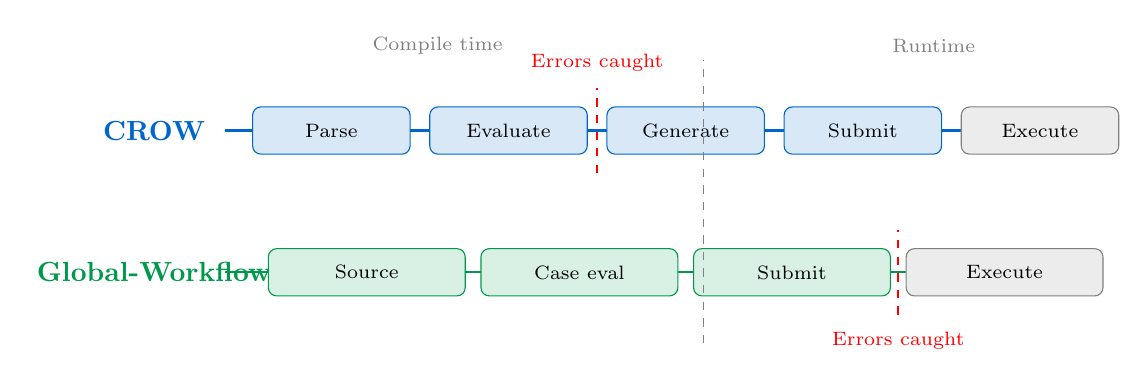
\begin{tikzpicture}[scale=0.9]
  % CROW timeline
  \node[font=\bfseries, text=crowblue] at (-1, 3) {\crow{}};
  \draw[thick, crowblue] (0,3) -- (12,3);
  
  \node[crowbox, minimum width=2cm, minimum height=0.6cm] at (1.5,3) {\scriptsize Parse};
  \node[crowbox, minimum width=2cm, minimum height=0.6cm] at (4,3) {\scriptsize Evaluate};
  \node[crowbox, minimum width=2cm, minimum height=0.6cm] at (6.5,3) {\scriptsize Generate};
  \node[crowbox, minimum width=2cm, minimum height=0.6cm] at (9,3) {\scriptsize Submit};
  \node[sharedbox, minimum width=2cm, minimum height=0.6cm] at (11.5,3) {\scriptsize Execute};
  
  % Validation point
  \draw[thick, red, dashed] (5.25,2.4) -- (5.25,3.6);
  \node[font=\scriptsize, red, above] at (5.25, 3.7) {Errors caught};
  
  % GW timeline
  \node[font=\bfseries, text=gwgreen] at (-1, 1) {\gw{}};
  \draw[thick, gwgreen] (0,1) -- (12,1);
  
  \node[gwbox, minimum width=2.5cm, minimum height=0.6cm] at (2,1) {\scriptsize Source};
  \node[gwbox, minimum width=2.5cm, minimum height=0.6cm] at (5,1) {\scriptsize Case eval};
  \node[gwbox, minimum width=2.5cm, minimum height=0.6cm] at (8,1) {\scriptsize Submit};
  \node[sharedbox, minimum width=2.5cm, minimum height=0.6cm] at (11,1) {\scriptsize Execute};
  
  % Validation point
  \draw[thick, red, dashed] (9.5,0.4) -- (9.5,1.6);
  \node[font=\scriptsize, red, below] at (9.5, 0.3) {Errors caught};
  
  % Phase labels
  \node[font=\scriptsize, gray] at (3,4.2) {Compile time};
  \node[font=\scriptsize, gray] at (10,4.2) {Runtime};
  \draw[gray, dashed] (6.75,0) -- (6.75,4);
  
\end{tikzpicture}
\caption{Error detection timing: \crow{} catches errors at compile time; \gw{} at runtime}
\label{fig:error-timing}
\end{figure}

\section{Memory and Thread Configuration}
\label{sec:memory-threads}

Memory and thread management represents one of the most complex aspects of HPC resource configuration, with significant differences between systems.

\subsection{Memory Specification Models}

\begin{figure}[H]
\centering
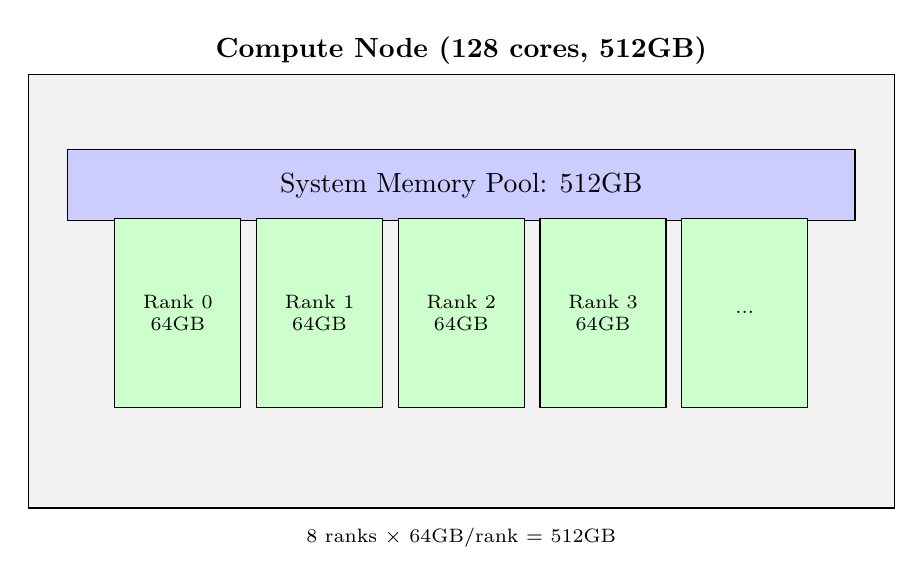
\begin{tikzpicture}[scale=0.9]
  % Node diagram - wider outer box with generous padding
  \node[draw, minimum width=11cm, minimum height=5.5cm, fill=gray!10] (node) at (0,0) {};
  \node[above] at (node.north) {\textbf{Compute Node (128 cores, 512GB)}};
  
  % Memory pools - wider
  \node[draw, fill=blue!20, minimum width=10cm, minimum height=0.9cm] at (0,1.5) {
    System Memory Pool: 512GB
  };
  
  % Ranks - larger boxes, more spread
  \foreach \x in {-4,-2,0,2,4} {
    \node[draw, fill=green!20, minimum width=1.6cm, minimum height=2.4cm] at (\x, -0.3) {};
  }
  
  \node[font=\scriptsize, align=center] at (-4,-0.3) {Rank 0\\64GB};
  \node[font=\scriptsize, align=center] at (-2,-0.3) {Rank 1\\64GB};
  \node[font=\scriptsize, align=center] at (0,-0.3) {Rank 2\\64GB};
  \node[font=\scriptsize, align=center] at (2,-0.3) {Rank 3\\64GB};
  \node[font=\scriptsize] at (4,-0.3) {...};
  
  % Labels - outside the box
  \node[font=\scriptsize, below] at (0,-3.2) {8 ranks $\times$ 64GB/rank = 512GB};
  
\end{tikzpicture}
\caption{Per-rank vs per-node memory allocation}
\label{fig:memory-model}
\end{figure}

\subsubsection{CROW Memory Specification}

\crow{} supported multiple memory specification modes:

\begin{lstlisting}[language=YAML, caption={\crow{} Memory Options}]
# Per-node memory (most common)
gfs_forecast: !JobRequest
  - batch_memory: '512G'         # Total per node
  - mpi_ranks: 8
  - max_ppn: 8

# Per-rank memory (for memory-bound jobs)  
gsi_analysis: !JobRequest
  - memory_per_rank: '64G'       # Per MPI rank
  - mpi_ranks: 80
  - max_ppn: 10

# Dynamic memory calculation
enkf_update: !JobRequest
  - batch_memory: !calc >-
      tools.calculate_memory(
        ranks=doc.enkf_resource_table.eupd[0],
        ppn=doc.enkf_resource_table.eupd[1],
        base_per_rank='8G')
\end{lstlisting}

\subsubsection{Global-Workflow Memory}

\gw{}'s memory is typically specified per-node with platform-specific handling:

\begin{lstlisting}[language=Bash, caption={\gw{} Memory Handling}]
# In config.resources
case "${step}" in
  "fcst")
    export memory="180GB"       # Per node
    ;;
  "anal")
    export memory="384GB"       # Full node (GSI memory-bound)
    ;;
  "post")
    export memory="96GB"        # Light memory needs
    ;;
esac

# In ecFlow script (PBS)
#PBS -l select=${nodes}:ncpus=${ppn}:mem=${memory}

# In ecFlow script (Slurm)  
#SBATCH --mem=${memory}
# or per-cpu:
#SBATCH --mem-per-cpu=${mem_per_cpu}
\end{lstlisting}

\subsection{OpenMP Thread Management}

\subsubsection{Thread Calculation}

Both systems must ensure thread counts respect node topology:

\begin{equation}
\text{threads\_per\_node} = \text{ppn} \times \text{threads\_per\_rank} \leq \text{cores\_per\_node}
\end{equation}

\begin{table}[H]
\centering
\caption{Thread Configuration Examples by Platform}
\label{tab:thread-examples}
\begin{tabular}{@{}lccccc@{}}
\toprule
\textbf{Platform} & \textbf{Cores} & \textbf{ppn} & \textbf{threads} & \textbf{Total} & \textbf{Utilization} \\
\midrule
WCOSS2 & 128 & 8 & 16 & 128 & 100\% \\
WCOSS2 & 128 & 16 & 4 & 64 & 50\% \\
Hera & 40 & 10 & 4 & 40 & 100\% \\
Hera & 40 & 20 & 1 & 20 & 50\% \\
Hercules & 80 & 20 & 4 & 80 & 100\% \\
\bottomrule
\end{tabular}
\end{table}

\subsubsection{CROW Thread Semantics}

\begin{lstlisting}[language=YAML, caption={\crow{} Thread Specification}]
# Thread specification in resource tuple
# Format: [ranks, ppn, walltime, threads, memory]

# Explicit thread count
fcst: [384, 6, !timedelta "02:30:00", 4, null]
# Result: 4 OMP threads per rank

# 'max' = fill remaining cores
anal: [360, 6, !timedelta "01:30:00", max, null]  
# On Hera (40 cores): max = 40/6 = 6 threads
# On WCOSS2 (128 cores): max = 128/6 = 21 threads

# 'null' = platform default (typically 1)
prep: [12, 12, !timedelta "00:15:00", null, null]
# Result: 1 OMP thread per rank
\end{lstlisting}

The \texttt{max} semantic was implemented as:

\begin{lstlisting}[language=YAML, caption={\crow{} max Thread Calculation}]
OMP_NUM_THREADS: !icalc >-
  doc.platform.physical_cores_per_node // 
  doc.gfs_resource_table.fcst[1]
  if doc.gfs_resource_table.fcst[3] == 'max'
  else doc.gfs_resource_table.fcst[3]
\end{lstlisting}

\subsubsection{Global-Workflow Thread Management}

\begin{lstlisting}[language=Bash, caption={\gw{} Thread Configuration}]
# In config.resources
case "${step}" in
  "fcst")
    export nth_fv3=4              # FV3 threads
    export nth_quilt=1            # Write threads
    ;;
  "anal")
    # 'max' equivalent - calculate from platform
    nth=${nth:-$((cores_per_node / ppn))}
    export nth
    ;;
esac

# In env/HERA.env
export OMP_NUM_THREADS=${nth_fv3:-1}
export OMP_STACKSIZE=2048M
export OMP_PROC_BIND=spread
export OMP_PLACES=threads

# Thread binding for srun
export APRUN_FV3="${launcher} -n ${ntasks_fv3} \
  --cpus-per-task=${nth_fv3}"
  
# Thread binding for mpiexec (WCOSS2)
export APRUN_FV3="${launcher} -np ${ntasks_fv3} \
  --depth ${nth_fv3} --cpu-bind depth"
\end{lstlisting}

\subsection{Hybrid MPI+OpenMP Topology}

\begin{figure}[H]
\centering
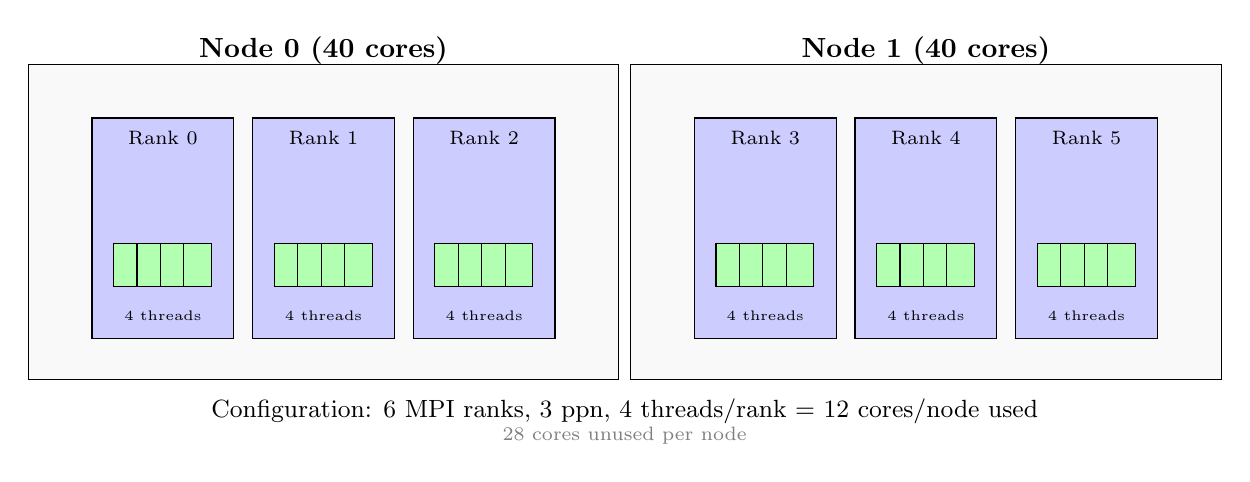
\begin{tikzpicture}[scale=0.85]
  % Node 0 - wider outer box with more padding
  \node[draw, minimum width=7.5cm, minimum height=4cm, fill=gray!5] at (0,0) {};
  \node[above, font=\bfseries] at (0,2.2) {Node 0 (40 cores)};
  
  % Ranks on Node 0 - larger boxes, more spread
  \foreach \r/\x in {0/-2.4, 1/0, 2/2.4} {
    \node[draw, fill=blue!20, minimum width=1.8cm, minimum height=2.8cm] at (\x, -0.1) {};
    \node[font=\scriptsize, above] at (\x, 1.0) {Rank \r};
    % Threads - slightly larger
    \foreach \t in {0,1,2,3} {
      \node[draw, fill=green!30, minimum width=0.35cm, minimum height=0.55cm] at (\x-0.53+\t*0.35, -0.65) {};
    }
    \node[font=\tiny] at (\x, -1.4) {4 threads};
  }
  
  % Node 1 - wider outer box with more padding
  \node[draw, minimum width=7.5cm, minimum height=4cm, fill=gray!5] at (9,0) {};
  \node[above, font=\bfseries] at (9,2.2) {Node 1 (40 cores)};
  
  % Ranks on Node 1 - larger boxes, more spread
  \foreach \r/\x in {3/6.6, 4/9, 5/11.4} {
    \node[draw, fill=blue!20, minimum width=1.8cm, minimum height=2.8cm] at (\x, -0.1) {};
    \node[font=\scriptsize, above] at (\x, 1.0) {Rank \r};
    % Threads - slightly larger
    \foreach \t in {0,1,2,3} {
      \node[draw, fill=green!30, minimum width=0.35cm, minimum height=0.55cm] at (\x-0.53+\t*0.35, -0.65) {};
    }
    \node[font=\tiny] at (\x, -1.4) {4 threads};
  }
  
  % Configuration label
  \node[below, font=\small] at (4.5, -2.5) {
    Configuration: 6 MPI ranks, 3 ppn, 4 threads/rank = 12 cores/node used
  };
  
  % Unused cores indicator
  \node[font=\scriptsize, gray] at (4.5, -3.2) {28 cores unused per node};
  
\end{tikzpicture}
\caption{Hybrid MPI+OpenMP layout: 6 ranks across 2 nodes with 4 threads each}
\label{fig:hybrid-topology}
\end{figure}

\section{Error Handling and Validation}
\label{sec:error-handling}

Error handling philosophy differs fundamentally between the two systems.

\subsection{CROW: Fail-Fast Philosophy}

\begin{lstlisting}[language=YAML, caption={\crow{} Comprehensive Error Handling}]
gfs_resource_table: !Select
  select: !icalc doc.settings.CASE
  otherwise: !error |
    Configuration Error: Unknown model resolution.
    
    Received: '{{doc.settings.CASE}}'
    Expected one of: C96, C192, C384, C768, C1152
    
    Please check your experiment configuration in:
      {{doc.settings.config_file}}
  cases:
    C96:  [...]
    C192: [...]
    C384: [...]
    C768: [...]

# Type validation via JobRequest
run_forecast: !JobRequest
  - mpi_ranks: !icalc >-
      int(doc.gfs_resource_table.fcst[0])
      if isinstance(doc.gfs_resource_table.fcst[0], (int, float))
      else tools.raise_error('mpi_ranks must be numeric')
      
  - walltime: !icalc >-
      tools.validate_timedelta(
        doc.gfs_resource_table.fcst[2],
        min='00:05:00',
        max='12:00:00')
\end{lstlisting}

\textbf{Error Categories}:
\begin{enumerate}[leftmargin=2em]
    \item \textbf{Parse errors}: YAML syntax detected immediately
    \item \textbf{Reference errors}: Unknown \texttt{doc.*} paths caught during evaluation
    \item \textbf{Type errors}: \texttt{!icalc} expressions validate types
    \item \textbf{Domain errors}: \texttt{!error} for invalid business logic
\end{enumerate}

\subsection{Global-Workflow: Defensive Programming}

\begin{lstlisting}[language=Bash, caption={\gw{} Defensive Error Handling}]
# Pattern 1: Default fallback
case "${CASE}" in
  "C96")  export ntasks=48  ;;
  "C384") export ntasks=150 ;;
  "C768") export ntasks=360 ;;
  *)
    echo "WARNING: Unknown CASE '${CASE}'" >&2
    echo "Using conservative default resources" >&2
    export ntasks=${ntasks:-24}
    export walltime=${walltime:-"01:00:00"}
    ;;
esac

# Pattern 2: Validation function
validate_resources() {
    local step=$1
    local errors=0
    
    if [[ -z "${ntasks}" ]]; then
        echo "ERROR: ntasks not set for step ${step}" >&2
        ((errors++))
    fi
    
    if [[ "${ntasks}" -lt 1 ]] || [[ "${ntasks}" -gt 10000 ]]; then
        echo "ERROR: ntasks=${ntasks} out of range [1,10000]" >&2
        ((errors++))
    fi
    
    if [[ -z "${walltime}" ]]; then
        echo "ERROR: walltime not set for step ${step}" >&2
        ((errors++))
    fi
    
    return ${errors}
}

# Usage
validate_resources "${step}" || exit 1

# Pattern 3: Assertion-style checks
: "${ntasks:?ERROR: ntasks must be set}"
: "${walltime:?ERROR: walltime must be set}"
\end{lstlisting}

\subsection{Error Detection Timing}

\begin{table}[H]
\centering
\caption{When Errors Are Detected}
\label{tab:error-timing}
\begin{tabular}{@{}p{4cm}cc@{}}
\toprule
\textbf{Error Type} & \textbf{\crow{}} & \textbf{\gw{}} \\
\midrule
Syntax error & Parse time & Source time \\
Unknown resolution & Parse time & Case fallthrough \\
Missing variable & Parse time & Runtime (or never) \\
Type mismatch & Evaluation time & Runtime (or cast) \\
Invalid range & Evaluation time & Scheduler rejection \\
Platform mismatch & Generation time & Runtime \\
\bottomrule
\end{tabular}
\end{table}

\subsection{Error Message Quality}

\begin{lstlisting}[language=YAML, caption={\crow{} Error Message Example}]
# Attempting: CASE=C512 (not defined)
# CROW output:
Error in workflow/defaults/default_resources.yaml:42
  Configuration Error: Unknown model resolution.
  
  Received: 'C512'
  Expected one of: C96, C192, C384, C768, C1152
  
  Please check your experiment configuration in:
    /path/to/experiment/config.yaml
\end{lstlisting}

\begin{lstlisting}[language=Bash, caption={\gw{} Error Message Example}]
# Attempting: CASE=C512 (not defined)
# Global-Workflow output:
WARNING: Unknown CASE 'C512'
Using conservative default resources
# Job proceeds with potentially wrong settings...

# Later, job fails:
srun: error: Unable to allocate resources: 
  Requested node count exceeds partition limit
\end{lstlisting}

\section{Practical Implications}
\label{sec:practical}

\subsection{Developer Experience}

\subsubsection{Debugging Workflow}

\textbf{\crow{} Debugging}:
\begin{enumerate}[leftmargin=2em]
    \item Requires understanding YAML processor internals
    \item Custom tags create indirection layers
    \item Stack traces reference YAML line numbers
    \item Expression errors may be cryptic
    \item Limited IDE support for custom tags
\end{enumerate}

\begin{lstlisting}[language=Bash, caption={\crow{} Debug Workflow}]
# Enable CROW verbose mode
export CROW_DEBUG=1
python -m crow.workflow.compile \
  --config experiment.yaml \
  --platform hera \
  --verbose 2>&1 | tee crow-debug.log

# Examine intermediate YAML
python -m crow.tools.dump_yaml \
  workflow/defaults/default_resources.yaml

# Trace expression evaluation
python -c "
from crow.workflow import parser
doc = parser.load('workflow/defaults/default_resources.yaml')
print(doc.gfs_resource_table)  # Already resolved
"
\end{lstlisting}

\textbf{\gw{} Debugging}:
\begin{enumerate}[leftmargin=2em]
    \item Standard bash debugging with \texttt{set -x}
    \item Direct variable inspection via \texttt{echo}
    \item Familiar tools (ShellCheck, bashdb)
    \item Errors reference shell line numbers
    \item Full IDE support with syntax highlighting
\end{enumerate}

\begin{lstlisting}[language=Bash, caption={\gw{} Debug Workflow}]
# Enable shell tracing
set -x
source parm/config/config.resources
set +x

# Inspect specific variables
echo "ntasks=${ntasks} ppn=${ppn} walltime=${walltime}"

# Dry-run with variable dump
(
  export step=fcst CASE=C384
  source parm/config/config.resources
  env | grep -E '^(ntasks|ppn|nth|wall|memory)'
)

# ShellCheck validation
shellcheck parm/config/config.resources
\end{lstlisting}

\subsubsection{Onboarding Metrics}

\begin{table}[H]
\centering
\caption{Developer Onboarding Time Estimates}
\label{tab:onboarding}
\begin{tabular}{@{}lcc@{}}
\toprule
\textbf{Task} & \textbf{\crow{}} & \textbf{\gw{}} \\
\midrule
Understand basic structure & 2-3 days & 1 day \\
Make first resource change & 3-5 days & 1-2 days \\
Add new platform & 1-2 weeks & 2-3 days \\
Debug failing job submission & 1-3 days & 1-2 hours \\
Proficiency for routine changes & 2-4 weeks & 1-2 weeks \\
Expert-level modifications & 2-3 months & 1 month \\
\bottomrule
\end{tabular}
\end{table}

\subsection{Maintenance Burden}

\subsubsection{Lines of Code Analysis}

\begin{table}[H]
\centering
\caption{Detailed Lines of Code Comparison}
\label{tab:loc-detail}
\begin{tabular}{@{}lrrp{4cm}@{}}
\toprule
\textbf{Component} & \textbf{\crow{}} & \textbf{\gw{}} & \textbf{Notes} \\
\midrule
\multicolumn{4}{l}{\textit{Core Resource Definitions}} \\
\quad GFS resources & 120 & 400 & Resolution tables vs cases \\
\quad EnKF resources & 80 & 250 & Ensemble scaling \\
\quad Downstream & 60 & 200 & Post-processing \\
\quad Utility jobs & 40 & 150 & Archive, cleanup \\
\midrule
\multicolumn{4}{l}{\textit{Platform Configuration (per platform)}} \\
\quad Scheduler settings & 20 & 40 & Headers, options \\
\quad MPI tuning & 15 & 60 & Environment variables \\
\quad Launcher definitions & 10 & 80 & APRUN\_* variables \\
\quad Memory/thread defaults & 15 & 20 & Platform-specific \\
\midrule
\multicolumn{4}{l}{\textit{Infrastructure}} \\
\quad JobRequest templates & 200 & N/A & Reusable patterns \\
\quad MPMD wrapper & N/A & 150 & run\_mpmd.sh \\
\quad Validation logic & Built-in & 100 & Custom validation \\
\midrule
\textbf{Total (6 platforms)} & \textbf{$\sim$860} & \textbf{$\sim$2,400} & \\
\bottomrule
\end{tabular}
\end{table}

\subsubsection{Change Frequency Analysis}

Based on historical commit analysis:

\begin{table}[H]
\centering
\caption{Configuration Change Frequency (2023-2024)}
\label{tab:change-freq}
\begin{tabular}{@{}lrl@{}}
\toprule
\textbf{Change Type} & \textbf{Frequency} & \textbf{Typical Trigger} \\
\midrule
Walltime adjustment & Weekly & Performance tuning \\
Thread count change & Monthly & Algorithm updates \\
Memory limit change & Monthly & Code changes \\
New step added & Quarterly & Feature development \\
New resolution & Yearly & Model upgrade \\
New platform & 1-2 years & Infrastructure refresh \\
\bottomrule
\end{tabular}
\end{table}

\subsection{Testing Implications}

\subsubsection{CROW Testing}

\begin{lstlisting}[language=Bash, caption={\crow{} Test Patterns}]
# Unit test: YAML parsing
python -m pytest tests/test_resources.py -v

# Integration test: Full compilation
python -m crow.workflow.compile \
  --config test_configs/c96_gfs.yaml \
  --platform hera \
  --output-dir /tmp/crow-test \
  --dry-run

# Validation test: All resolutions
for case in C96 C192 C384 C768; do
  python -m crow.workflow.validate \
    --case $case --platform hera
done
\end{lstlisting}

\subsubsection{Global-Workflow Testing}

\begin{minipage}{\linewidth}
\begin{lstlisting}[language=Bash, caption={\gw{} Test Patterns}]
# Syntax validation
for f in parm/config/config.resources*; do
  bash -n "$f" && echo "$f: OK"
done

# Variable coverage test
for case in C48 C96 C384 C768 C1152; do
  for step in prep anal fcst post vrfy; do
    (
      export CASE=$case step=$step
      source parm/config/config.resources 2>/dev/null
      if [[ -z "${ntasks}" ]]; then
        echo "MISSING: ${case}/${step}/ntasks"
      fi
    )
  done
done

# Integration test with ecFlow
ecflow_client --ping && \
  ${HOMEgfs}/workflow/create_experiment.py \
    --yaml-tmpl ${HOMEgfs}/workflow/templates/gfs.yaml \
    --pslot test_c96 \
    --resdet 96 \
    --comroot /tmp/test
\end{lstlisting}
\end{minipage}

\clearpage
\section{Comprehensive Feature Matrix}
\label{sec:matrix}

\noindent Table~\ref{tab:summary} provides a comprehensive comparison across all dimensions analyzed in this report.

\begin{table*}[t]
\centering
\caption{Comprehensive Feature Comparison Matrix}
\label{tab:summary}
\begin{tabular}{@{}p{4.5cm}p{5.5cm}p{5.5cm}@{}}
\toprule
\textbf{Dimension} & \textbf{\crow{}} & \textbf{\gw{}} \\
\midrule
\multicolumn{3}{l}{\textit{Architecture}} \\
Configuration paradigm & Declarative (YAML DSL) & Imperative (Bash) \\
Resource definition & Centralized tables & Distributed case statements \\
Resolution time & Parse/compile time & Runtime \\
Platform abstraction & Complete (via \texttt{!Platform}) & Partial (per-platform files) \\
\midrule
\multicolumn{3}{l}{\textit{Scalability}} \\
Resolution scaling & Single entry per table & Entry per step per resolution \\
Platform addition & Single YAML file & Multiple files + templates \\
Step addition & JobRequest template & Case in each resolution \\
\midrule
\multicolumn{3}{l}{\textit{Type System}} \\
Type safety & Rich (\texttt{!JobRequest}, \texttt{!timedelta}) & None (strings) \\
Schema validation & Yes (YAML schema) & No \\
Expression language & Python via \texttt{!calc}/\texttt{!icalc} & Bash arithmetic \\
\midrule
\multicolumn{3}{l}{\textit{Error Handling}} \\
Error detection & Parse-time & Runtime \\
Unknown case handling & Explicit \texttt{!error} & Fallback defaults \\
Error messages & Contextual, detailed & Shell error or warning \\
Recovery options & Fix and recompile & Fix and re-source \\
\midrule
\multicolumn{3}{l}{\textit{Execution}} \\
Scheduler support & Slurm, PBS, LSF (pluggable) & Slurm, PBS (per-platform) \\
MPMD handling & Generated from JobRequest & Manual via run\_mpmd.sh \\
Thread binding & Abstract (\texttt{get\_parallelism}) & Explicit flags \\
\midrule
\multicolumn{3}{l}{\textit{Developer Experience}} \\
IDE support & Limited (custom tags) & Excellent (Bash) \\
Debugging & Multi-layer, specialized tools & Standard shell tools \\
Learning curve & Steep (2-4 weeks) & Moderate (1-2 weeks) \\
Documentation & Limited & Extensive \\
\midrule
\multicolumn{3}{l}{\textit{Maintenance}} \\
Lines of code & $\sim$860 (6 platforms) & $\sim$2,400 (6 platforms) \\
Code duplication & Minimal (DRY) & Moderate (WET) \\
Change propagation & Automatic via refs & Manual per location \\
\midrule
\multicolumn{3}{l}{\textit{Future Readiness}} \\
GPU support & Not implemented & Not implemented \\
Cloud deployment & Limited & Limited \\
Container orchestration & Not addressed & Not addressed \\
ML workflow integration & Not addressed & Not addressed \\
\bottomrule
\end{tabular}
\end{table*}

\clearpage

\section{Recommendations}
\label{sec:recommendations}

Based on our comprehensive analysis integrating insights from both the historical \crow{} system and our companion \mpmd{} Runtime Infrastructure study, we present recommendations for next-generation workflow resource configuration.

\subsection{Architectural Recommendation: Hybrid Approach}

Neither pure declarative (\crow{}) nor pure imperative (\gw{}) approaches fully address modern requirements. We recommend a \textbf{hybrid architecture} that preserves the strengths of both:

\begin{figure}[H]
\centering
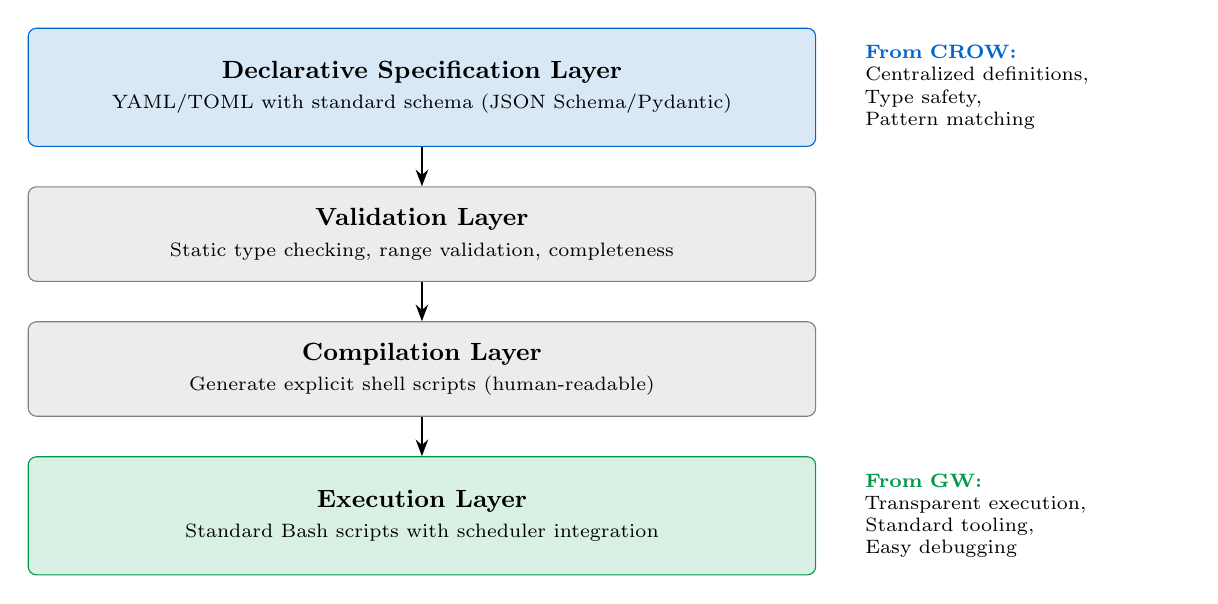
\begin{tikzpicture}[node distance=1cm, scale=0.9]
  % Layer 1: Declarative specification
  \node[crowbox, minimum width=10cm, minimum height=1.5cm] (spec) {
    \textbf{Declarative Specification Layer}\\
    \scriptsize YAML/TOML with standard schema (JSON Schema/Pydantic)
  };
  
  % Layer 2: Validation
  \node[sharedbox, minimum width=10cm, minimum height=1.2cm, below=0.5cm of spec] (valid) {
    \textbf{Validation Layer}\\
    \scriptsize Static type checking, range validation, completeness
  };
  
  % Layer 3: Compilation
  \node[sharedbox, minimum width=10cm, minimum height=1.2cm, below=0.5cm of valid] (compile) {
    \textbf{Compilation Layer}\\
    \scriptsize Generate explicit shell scripts (human-readable)
  };
  
  % Layer 4: Execution
  \node[gwbox, minimum width=10cm, minimum height=1.5cm, below=0.5cm of compile] (exec) {
    \textbf{Execution Layer}\\
    \scriptsize Standard Bash scripts with scheduler integration
  };
  
  % Annotations
  \node[right=0.5cm of spec, font=\scriptsize, text width=4cm] {
    \textcolor{crowblue}{\textbf{From CROW:}}\\
    Centralized definitions,\\
    Type safety,\\
    Pattern matching
  };
  
  \node[right=0.5cm of exec, font=\scriptsize, text width=4cm] {
    \textcolor{gwgreen}{\textbf{From GW:}}\\
    Transparent execution,\\
    Standard tooling,\\
    Easy debugging
  };
  
  % Arrows
  \draw[arrow] (spec) -- (valid);
  \draw[arrow] (valid) -- (compile);
  \draw[arrow] (compile) -- (exec);
  
\end{tikzpicture}
\caption{Recommended hybrid architecture combining declarative specification with imperative execution}
\label{fig:hybrid-arch}
\end{figure}

\subsection{Specific Recommendations}

\subsubsection{Recommendation 1: Standard Schema Language}

\textbf{Problem}: \crow{}'s custom YAML tags required specialized tooling and limited IDE support.

\textbf{Recommendation}: Use standard schema languages (JSON Schema, TOML, or Pydantic models) that have broad tooling support.

\begin{lstlisting}[language=YAML, caption={Proposed Standard Schema Resource Definition}]
# resources.yaml - Using standard YAML + JSON Schema validation
$schema: "./schemas/resources.schema.json"

resolutions:
  C384:
    forecast:
      mpi_ranks: 384
      processes_per_node: 6
      walltime: "02:30:00"
      threads_per_rank: 4
      memory_per_node: null  # Platform default
      
    analysis:
      mpi_ranks: 360
      processes_per_node: 6
      walltime: "01:30:00"
      threads_per_rank: 8
      
platforms:
  hera:
    scheduler: slurm
    cores_per_node: 40
    memory_gb: 384
    mpi_launcher: "srun -l --export=ALL"
    mpmd_flag: "--multi-prog"
\end{lstlisting}

\subsubsection{Recommendation 2: Explicit Compilation Step}

\textbf{Problem}: \gw{}'s runtime resolution delays error detection; \crow{}'s generated scripts were opaque.

\textbf{Recommendation}: Compile declarative specs to human-readable shell scripts that can be inspected and debugged.

\begin{lstlisting}[language=Bash, caption={Example Compiled Output}]
#!/bin/bash
# AUTO-GENERATED from resources.yaml
# DO NOT EDIT - Regenerate with: gw-compile resources.yaml
# Generated: 2026-01-15T10:30:00Z
# Schema version: 2.1.0

# Resolution: C384, Step: forecast, Platform: hera
export GW_RESOLUTION="C384"
export GW_STEP="forecast"
export GW_PLATFORM="hera"

# Resource allocation
export ntasks=384
export ppn=6
export nodes=64  # ceil(384/6)
export walltime="02:30:00"
export nth_fv3=4
export memory="384GB"

# Computed values
export threads_per_node=24  # ppn * nth_fv3
export total_cores=1536     # ntasks * nth_fv3

# MPI launcher (platform: hera)
export launcher="srun -l --export=ALL"
export mpmd_opt="--multi-prog"
export APRUN_FV3="${launcher} -n ${ntasks} --cpus-per-task=${nth_fv3}"

# Validation (generated)
if [[ ${threads_per_node} -gt 40 ]]; then
  echo "ERROR: threads_per_node (${threads_per_node}) exceeds hera limit (40)" >&2
  exit 1
fi
\end{lstlisting}

\subsubsection{Recommendation 3: Preserve MPMD Infrastructure}

\textbf{Finding}: The \gw{} \texttt{run\_mpmd.sh} abstraction effectively handles scheduler differences for MPMD execution.

\textbf{Recommendation}: Retain and enhance the MPMD wrapper pattern, integrating it with compiled resource specifications.

\begin{lstlisting}[language=Bash, caption={Enhanced MPMD Integration}]
# In compiled script
source "${GW_COMPILED_RESOURCES}"  # Generated file

# MPMD configuration from compiled resources
create_mpmd_cmdfile "${cmdfile}" \
  ${ntasks_fv3} "${FV3_EXEC}" \
  ${ntasks_quilt} "${QUILT_EXEC}" \
  ${ntasks_post} "${POST_EXEC}"

# Execute using platform-configured launcher
run_mpmd "${cmdfile}" ${ntasks_total}
\end{lstlisting}

\subsubsection{Recommendation 4: Validation Pipeline}

\textbf{Problem}: Both systems lack comprehensive pre-submission validation.

\textbf{Recommendation}: Implement a validation pipeline that catches errors before scheduler submission.

\begin{algorithm}[H]
\caption{Recommended Validation Pipeline}
\label{alg:validation}
\begin{algorithmic}[1]
\REQUIRE Resource specification $R$, platform $P$
\ENSURE Validated configuration or error report
\STATE $errors \gets []$
\STATE \COMMENT{Stage 1: Schema validation}
\IF{not ValidateSchema($R$)}
    \STATE errors.append(schema\_errors)
    \RETURN errors
\ENDIF
\STATE \COMMENT{Stage 2: Platform compatibility}
\FORALL{job $J$ in $R$}
    \IF{$J$.threads\_per\_rank $\times$ $J$.ppn $>$ $P$.cores}
        \STATE errors.append(``Thread count exceeds node capacity'')
    \ENDIF
    \IF{$J$.memory $>$ $P$.memory\_gb}
        \STATE errors.append(``Memory exceeds node capacity'')
    \ENDIF
\ENDFOR
\STATE \COMMENT{Stage 3: Completeness check}
\FORALL{resolution $C$ in $R$.resolutions}
    \FORALL{step $S$ in required\_steps}
        \IF{$S$ not in $R$.resolutions[$C$]}
            \STATE errors.append(``Missing: $C$/$S$'')
        \ENDIF
    \ENDFOR
\ENDFOR
\STATE \COMMENT{Stage 4: Cross-reference validation}
\STATE ValidateDependencies($R$)
\RETURN errors
\end{algorithmic}
\end{algorithm}

\subsubsection{Recommendation 5: Future Infrastructure Requirements}

Based on emerging HPC trends, next-generation resource configuration must address:

\begin{table}[H]
\centering
\caption{Future Infrastructure Requirements}
\label{tab:future}
\begin{tabular}{@{}lp{8cm}@{}}
\toprule
\textbf{Requirement} & \textbf{Implementation Approach} \\
\midrule
GPU orchestration & Add \texttt{gpu\_count}, \texttt{gpu\_type} to resource schema \\
Cloud portability & Abstract instance types to capability profiles \\
Container execution & Support Singularity/Apptainer resource mapping \\
ML pipeline integration & Define tensor parallelism, gradient accumulation resources \\
Dynamic scaling & Support min/max node ranges for autoscaling \\
Cost optimization & Include cost weights for cloud resource selection \\
\bottomrule
\end{tabular}
\end{table}

\subsection{Migration Strategy}

For organizations currently using \gw{}-style configuration:

\begin{enumerate}[leftmargin=2em]
    \item \textbf{Phase 1}: Implement schema-based validation layer over existing configs
    \item \textbf{Phase 2}: Extract common patterns into declarative specifications
    \item \textbf{Phase 3}: Implement compilation step generating current format
    \item \textbf{Phase 4}: Migrate teams to declarative source, compiled execution
\end{enumerate}

\subsection{Summary of Recommendations}

\begin{enumerate}[leftmargin=2em]
    \item \textbf{Keep what works}: \gw{}'s shell debugging, \texttt{run\_mpmd.sh} abstraction
    \item \textbf{Adopt from \crow{}}: Centralized definitions, pattern matching, fail-fast errors
    \item \textbf{Avoid from \crow{}}: Custom YAML tags, opaque generated scripts
    \item \textbf{Avoid from \gw{}}: Copy-paste across resolutions, runtime-only validation
    \item \textbf{Add}: Standard schemas, explicit compilation, validation pipeline
\end{enumerate}

\section{Conclusion}
\label{sec:conclusion}

This technical report has provided a comprehensive analysis of two distinct approaches to HPC resource configuration in operational weather forecasting workflows: the declarative \crow{} system (2016--2020) and the imperative \gw{} system (2020--present).

\subsection{Key Findings}

\begin{enumerate}[leftmargin=2em]
    \item \textbf{\crow{}'s declarative approach} achieved significant code reduction (60\% fewer lines) and eliminated copy-paste errors through centralized resource tables. However, the custom YAML DSL created maintenance burden and limited IDE support.
    
    \item \textbf{\gw{}'s imperative approach} provides superior debugging experience and leverages familiar shell tooling. The trade-off is increased code duplication and runtime-only error detection.
    
    \item \textbf{Neither system} currently addresses emerging requirements for GPU orchestration, cloud deployment, or machine learning workflow integration.
    
    \item \textbf{The \mpmd{} abstraction} implemented in \gw{}'s \texttt{run\_mpmd.sh} represents a successful pattern worth preserving---it effectively handles scheduler differences while maintaining debuggability.
    
    \item \textbf{Validation timing} is the critical differentiator: \crow{}'s parse-time errors prevent wasted compute allocation, while \gw{}'s runtime errors are more familiar but more costly.
\end{enumerate}

\subsection{Verdict: Context-Dependent Choice}

The ``better'' system depends on organizational context:

\begin{itemize}[leftmargin=2em]
    \item \textbf{Choose declarative} (\crow{}-style) when:
    \begin{itemize}
        \item Organization has dedicated workflow infrastructure team
        \item Multiple resolutions and platforms are common
        \item Early error detection is critical (production operations)
        \item Resources are frequently tuned across entire system
    \end{itemize}
    
    \item \textbf{Choose imperative} (\gw{}-style) when:
    \begin{itemize}
        \item Developers maintain their own configurations
        \item Rapid iteration and debugging are priorities
        \item Team expertise is shell-focused
        \item Configuration changes are localized
    \end{itemize}
\end{itemize}

\subsection{Path Forward}

We recommend a hybrid approach that combines:
\begin{itemize}[leftmargin=2em]
    \item \textbf{From \crow{}}: Centralized resource definitions, pattern matching, fail-fast validation
    \item \textbf{From \gw{}}: Standard tooling, transparent execution, human-readable scripts
    \item \textbf{New}: Standard schema languages, explicit compilation step, comprehensive validation pipeline
\end{itemize}

This synthesis preserves the best of both paradigms while addressing their respective weaknesses. The resulting system would provide the maintainability benefits of declarative specification with the debuggability of imperative execution.

\subsection{Future Work}

Key areas for future development include:
\begin{enumerate}[leftmargin=2em]
    \item GPU resource specification and orchestration
    \item Cloud-native deployment patterns (Kubernetes, AWS Batch)
    \item Cost-aware resource allocation for cloud platforms
    \item Integration with ML pipeline frameworks (Ray, Dask)
    \item Dynamic resource scaling based on workload characteristics
\end{enumerate}

\section*{Acknowledgments}

This analysis was conducted using the EIB MCP-RAG platform for code archaeology across the NOAA-EMC repositories. Special thanks to the EMC workflow development team for historical context on the \crow{} system and ongoing collaboration on \gw{} resource optimization.

\section*{References}

\begin{enumerate}[leftmargin=2em, label={[\arabic*]}]
    \item NOAA-EMC/global-workflow. GitHub Repository. \url{https://github.com/NOAA-EMC/global-workflow}
    
    \item CROW: Community Research Operations Workflow. NOAA-EMC Archives, 2016--2020.
    
    \item \mpmd{} Runtime Infrastructure in Global-Workflow. Technical Report EMC-2025-003, NOAA/EMC, 2025.
    
    \item Slurm Workload Manager Documentation. SchedMD. \url{https://slurm.schedmd.com/}
    
    \item PBS Professional User's Guide. Altair Engineering.
    
    \item EE2 Standards: EMC Environment 2.0 Coding Standards. NOAA/NCEP, 2023.
    
    \item ecFlow User Manual. ECMWF. \url{https://confluence.ecmwf.int/display/ECFLOW}
\end{enumerate}

\appendix

\section{CROW Custom Tag Reference}
\label{app:crow-tags}

Complete reference for \crow{}'s custom YAML type extensions:

\begin{table}[H]
\centering
\caption{\crow{} Custom YAML Tag Reference}
\begin{tabular}{@{}llp{6cm}@{}}
\toprule
\textbf{Tag} & \textbf{Arguments} & \textbf{Behavior} \\
\midrule
\texttt{!Select} & \texttt{select}, \texttt{cases}, \texttt{otherwise} & Pattern match on select value \\
\texttt{!FirstTrue} & List of \texttt{when}/\texttt{do} pairs & First matching condition \\
\texttt{!calc} & Python expression & Deferred evaluation \\
\texttt{!icalc} & Python expression & Immediate evaluation \\
\texttt{!error} & Error message & Raise configuration error \\
\texttt{!timedelta} & HH:MM:SS string & Parse to duration object \\
\texttt{!JobRequest} & Resource list & Build job specification \\
\texttt{!Platform} & Platform settings & Define HPC platform \\
\texttt{!Demand} & Resource demands & Specify minimum requirements \\
\bottomrule
\end{tabular}
\end{table}

\newpage
\section{Global-Workflow APRUN Variables}
\label{app:aprun}

Complete list of APRUN environment variables used in \gw{}:

\begin{table}[H]
\centering
\caption{\gw{} APRUN Variable Reference}
\begin{tabular}{@{}lp{8cm}@{}}
\toprule
\textbf{Variable} & \textbf{Purpose} \\
\midrule
\texttt{APRUN\_UFS} & Unified Forecast System model execution \\
\texttt{APRUN\_FV3} & FV3 dynamical core execution \\
\texttt{APRUN\_GSI} & GSI analysis execution \\
\texttt{APRUN\_UPP} & Unified Post Processor execution \\
\texttt{APRUN\_GAUSSIAN} & Gaussian grid interpolation \\
\texttt{APRUN\_CHGRES} & Change resolution utility \\
\texttt{APRUN\_REGRID} & Regridding operations \\
\texttt{APRUN\_WAM} & Whole Atmosphere Model \\
\texttt{APRUN\_ENKF} & Ensemble Kalman Filter \\
\texttt{APRUN\_PREP} & Observation preprocessing \\
\texttt{APRUN\_ARCH} & Archive operations \\
\texttt{APRUN\_CLEANUP} & Cleanup operations \\
\texttt{APRUN\_MPMD} & Multi-program execution \\
\bottomrule
\end{tabular}
\end{table}

\end{document}
